\chapter{La modélisation du carrefour}

\label{chap:modelisation}

% Intro du chapitre : ma modélisation est basée sur OSM donc je décris ce que contient OSM

Le carrefour peut être un espace d'interaction entre piétons et véhicules. Dans le cas où il permet à un piéton de le franchir, la signalisation permet alternativement aux flux des piétons ou des voitures de le traverser en sécurité. Pour une \gls{pcdv}, cette traversée peut être complexe en raison de la variabilité et l'hétérogénéité des configurations, du nombre de voies présentes, et des équipements de contrôle du trafic et d'accessibilité. Dans ce chapitre, nous présentons l'architecture du carrefour du point de vue d'une personne concernée, puis nous analysons au regard des besoins évoqués la manière dont ces données sont représentées dans la base de données \gls{osm}. Enfin, nous proposons une représentation objet de la donnée \gls{osm} que nous appliquons à une modélisation du carrefour orientée sur l'accessibilité.

% Un "état de l'art" à la JLZ pour chaque sous-partie : une vue précise du carrefour, de son infrastructure et des éléments d'accessibilité qui le compose.
% Penser le carrefour du point de vue du piéton sous la forme d'un graphe 

\section{La structure globale du carrefour}

% Pour définir les éléments de mon modèle, j'ai utilisé des méthodo de travail : je suis allé interroger des professionnels, etc. Mentionner le fait d'être allé rencontrer des personnes du CRDV, autres professionnels.

Un carrefour, tel que défini par le dictionnaire Larousse, est un \pquote{lieu où se croisent plusieurs rues ou plusieurs routes, généralement aménagé en vue d'éviter les risques de collision, et parfois d'améliorer le débit}. Une particularité concernant nos travaux est que le carrefour nous intéresse du point de vue du piéton, et notamment du piéton concerné par la déficience visuelle, dont les spécificités doivent être prise en compte dans la définition d'un carrefour tel que nous le concevons. Lors des travaux préliminaires à ce mémoire, nous avons interrogé des personnes concernées et professionnels du \gls{crdv} de Clermont-Ferrand pour établir cette définition. Pour ces dernières, la limite d'un carrefour correspond à l'étendue de ce qu'une personne peut entendre. Bien qu'il existe des travaux de modélisation accoustique \cite{Bullen1977} orientés notamment sur la propagation du bruit, cette approche nous semble difficile à généraliser dans un premier temps. Nous avons donc choisi de nous concentrer tout d'abord sur la structure du carrefour du point de vue du piéton, en en proposant une représentation sous forme de graphe, puis en s'intéressant aux élements d'accessibilité spécifiques à la mobilité des \glspl{pcdv}.

\subsection{Le graphe du carrefour du point de vue d'un piéton}

\label{sec:modelisation_definitions}

Pour modéliser le carrefour du point de vue d'un piéton, nous avons choisi de nous reposer sur une approche graphe afin de le définir et de le délimiter dans un réseau routier. Les définitions suivantes en définissent la structure :

\begin{definition}
    On appelle \textbf{couverture} d'un graphe $G_0 = (V_0,E_0)$ et plongé dans le plan un ensemble de sous-graphes $\mathcal{G_0}$ tels que:
    \begin{itemize}
        \item Si $G_1=(V_1, E_1) \in \mathcal{G_0}$ et $G_2=(V_2, E_2) \in \mathcal{G_p}$, alors $E_1 \cap E_2 = \emptyset$
        \item $\forall e \in E_p$, $\exists!~G_1=(V_1, E_1) \in \mathcal{G_p}$ tel que $e \in E_1$
    \end{itemize}
    
    Dans la suite, on appelle $\mathcal{G}_p$ une couverture du graphe piéton, et $\mathcal{G}_r$ une couverture du graphe routier.
    
    Dans la suite, on dira que deux sous-graphes sont \textbf{connectés} s'ils partagent au moins un sommet en commun.
\end{definition}

\begin{definition}
    On défini un \textbf{graphe multimodal} comme un graphe $G = (V,E)$ plongé dans le plan et muni d'une couverture $\{G_r=(V_r, E_r), G_p = (V_p, E_p)\}$ composée d'un \textbf{graphe routier} $G_r$ et d'un \textbf{graphe piéton} $G_p$.

    Dans la suite, on note $G = (V,E)$ un graphe multimodal sur lequel on défini les autres ensembles et propriétés.
\end{definition}

\noindent
Remarque: l'intersection entre $V_r$ et $V_p$ peut ne pas être vide.

\begin{definition}
    Soient $G_1=(V_1, E_1)$ et $G_2=(V_2, E_2)$ deux sous-graphes de $G=(V, E)$.
    
    On appelle \textbf{fonction d'association} $f: E_1 \rightarrow E_2$ toute fonction qui à chaque arête de $G_1$ associe une arête de $G_2$.
\end{definition}

\begin{definition}
    Alors on appelle \textbf{trottoir} tout $G_t = (V_t, E_t)\in \mathcal{G}_p$ sous-graphe du graphe piéton muni d'une fonction d'association $f_t: G_t \rightarrow G_r$ projetant les arêtes de $G_t$ dans le graphe routier. Cette fonction $f_t$ est appelée \textbf{fonction d'adjacence} du trottoir $G_t$.

    On note $\mathcal{G}_t$ l'ensemble des trottoirs.
\end{definition}

\begin{definition}
    Étant donné une couverture $\mathcal{G}_p$ d'un graphe piéton $G_p$, un ensemble de fonctions d'adjacence est dit \textbf{un ensemble de trottoirs couvrants} s'il n'existe pas de sommet $v \in G_p$ appartenant à plus d'un trottoir.
\end{definition}

\noindent
Exemple: couverture d'un graphe piéton qui n'est pas un ensemble de trottoirs couvrants (voir Figure \ref{fig:mod_ex_trottoirs_couvrants}).

\begin{figure}
    \centering
    
\includegraphics{images/placeholder.jpg}
    \caption{Ces deux trottoirs ne sont pas couvrants car ils possèdent un noeud en commun.}
    \label{fig:mod_ex_trottoirs_couvrants}
\end{figure}

\begin{definition}
    On appelle \textbf{chemin} un graphe $G_{ch} = (V_{ch}, E_{ch})$ tel que $V_{ch}=\{p_1,p_2,\dots,p_n\}$ et $E_{ch}=\{\{p_1,p_2\},\{p_2,p_3\},\dots,\{p_{n-1},p_n\}\}$.
\end{definition}

\begin{definition}
    Un \textbf{passage piéton} $G_{pp} = (V_{pp}, E_{pp}) \in \mathcal{G}_p$ est un chemin $(p_1, p_2,\dots, p_n)$ tel que:

    \begin{itemize}
        \item $p_2, p_3, \dots, p_{n-1}$ sont inclus dans le graphe routier
        \item $p_2, p_3, \dots, p_{n-1}$ n'appartiennent pas à un trottoir
        \item $p_1$ et $p_n$ appartiennent chacun à un trottoir
    \end{itemize}
\end{definition}

\begin{definition}
    Une couverture $\mathcal{G}_r$ d'un réseau routier est dite \textbf{couverture routière complète} si et seulement si elle est composée d'une union disjointe de \textbf{coeurs de carrefours} $\mathcal{G}_c \subset \mathcal{G}_r$ et de \textbf{branches} $\mathcal{G}_b \subset \mathcal{G}_r$ tels que:

    \begin{itemize}
        \item $\mathcal{G}_c \neq \emptyset$ 
        \item Deux coeurs de carrefour ne sont pas connectés
        \item Chaque branche est connectée à un ou deux coeurs de carrefour
        \item Un coeur de carrefour est au minimum connecté à deux branches distinctes
    \end{itemize}
    \label{def:modelisation_couverture_routiere_complète}
\end{definition}

\noindent
Remarque: un cœur de carrefour ne peut pas être un chemin.

\noindent
Exemples:
\begin{itemize}
    \item Une couverture routière qui n'est pas complète (voir Figure \ref{fig:mod_ex_couverture_routiere_incomplete})
    \item Une couverture routière à plusieurs carrefours, dites de quartier (voire Figure \ref{fig:mod_ex_couverture_routiere_quartier})
\end{itemize}

\begin{figure}
    \centering
    \begin{subfigure}[t]{.49\linewidth}
        
\includegraphics[width=\textwidth]{images/placeholder.jpg}
        \caption{Couverture routière incomplète: deux branches ne peuvent pas être connectées.\label{fig:mod_ex_couverture_routiere_incomplete}}
    \end{subfigure}
    \begin{subfigure}[t]{.49\linewidth}
        
\includegraphics[width=\textwidth]{images/placeholder.jpg}
        \caption{Une couverture de quartier comprend plusieurs carrefours. \label{fig:mod_ex_couverture_routiere_carrefour}}
    \end{subfigure}
    \caption{On remarque la différence entre une couverture routière incomplète et une couverture routière complète.}
    \label{fig:mod_ex_couverture_routiere_quartier}
\end{figure}

\begin{definition}
    Une couverture $\mathcal{G}_p$ d'un réseau piéton est dite \textbf{couverture piétonne complète} si et seulement si elle est composée d'une union disjointe de trottoirs, de passages piétons, et d'\textbf{îlots} $\mathcal{G}_i \in \mathcal{G}_p$ tel qu'un îlot n'est connecté qu'à des passages piéton.
\end{definition}

\begin{definition}
    Une \textbf{traversée} $G_{t} = (V_{t}, E_{t}) \in \mathcal{G}_p$ est un chemin $(p_1, p_2,\dots, p_n)$ tel que:

    \begin{itemize}
        \item $p_1$ et $p_n$ appartiennent à un trottoir
        \item $p_2, p_3, \dots, p_{n-1}$ n'appartiennent pas à un trottoir
        \item $\forall e \in E_t$, $e$ appartient soit à un passage piéton, soit à un îlot
    \end{itemize}
\end{definition}

\begin{definition}
    Un \textbf{carrefour} est un graphe multimodal composé d'une couverture routière complète ne contenant qu'un seul cœur de carrefour, d'une couverture piétonne complète et d'un ensemble de traversées (voir Figure \ref{fig:mod_ex_graphe_carrefour}).
\end{definition}

\begin{figure}
    \centering
    
\includegraphics{images/placeholder.jpg}
    \caption{Le graphe multimodal d'un carrefour.}
    \label{fig:mod_ex_graphe_carrefour}
\end{figure}

\subsection{Les repères au sein du carrefour}

\label{sec:mod_repere_carrefour}

Pour effectuer une traversée du carrefour en sécurité, il existe un certain nombre d'équipements d'accessibilité pouvant être mobilisés par une \gls{pcdv}. Ces équipements ont des rôles divers, comme permettre de repérer une traversée, ou d'y accéder par un nivellement adapté (dans le cas d'une \gls{pmr} par exemple). Pour répondre aux besoins des différents usagers, ces équipements font appel à des sens différents: l'ouïe pour les signaux sonores, le toucher pour les éléments tactiles, mais également la vue pour les potelets contrastés ou les passages piétons matérialisés par de la pleinture au sol qui peut être mobilisée par les \glspl{pcdv} présentant un résidu visuel. Plusieurs équipements pouvant être rencontrés sur un carrefour sont présentés au sein de la table \ref{tab:modelisation_objets}.

\begin{table}
    \begin{center}
    \scriptsize
    \begin{tabular}{ | m{2cm} | m{10cm} }
        Image & Description \tabularnewline
        \hline
        \resizebox{2cm}{!}{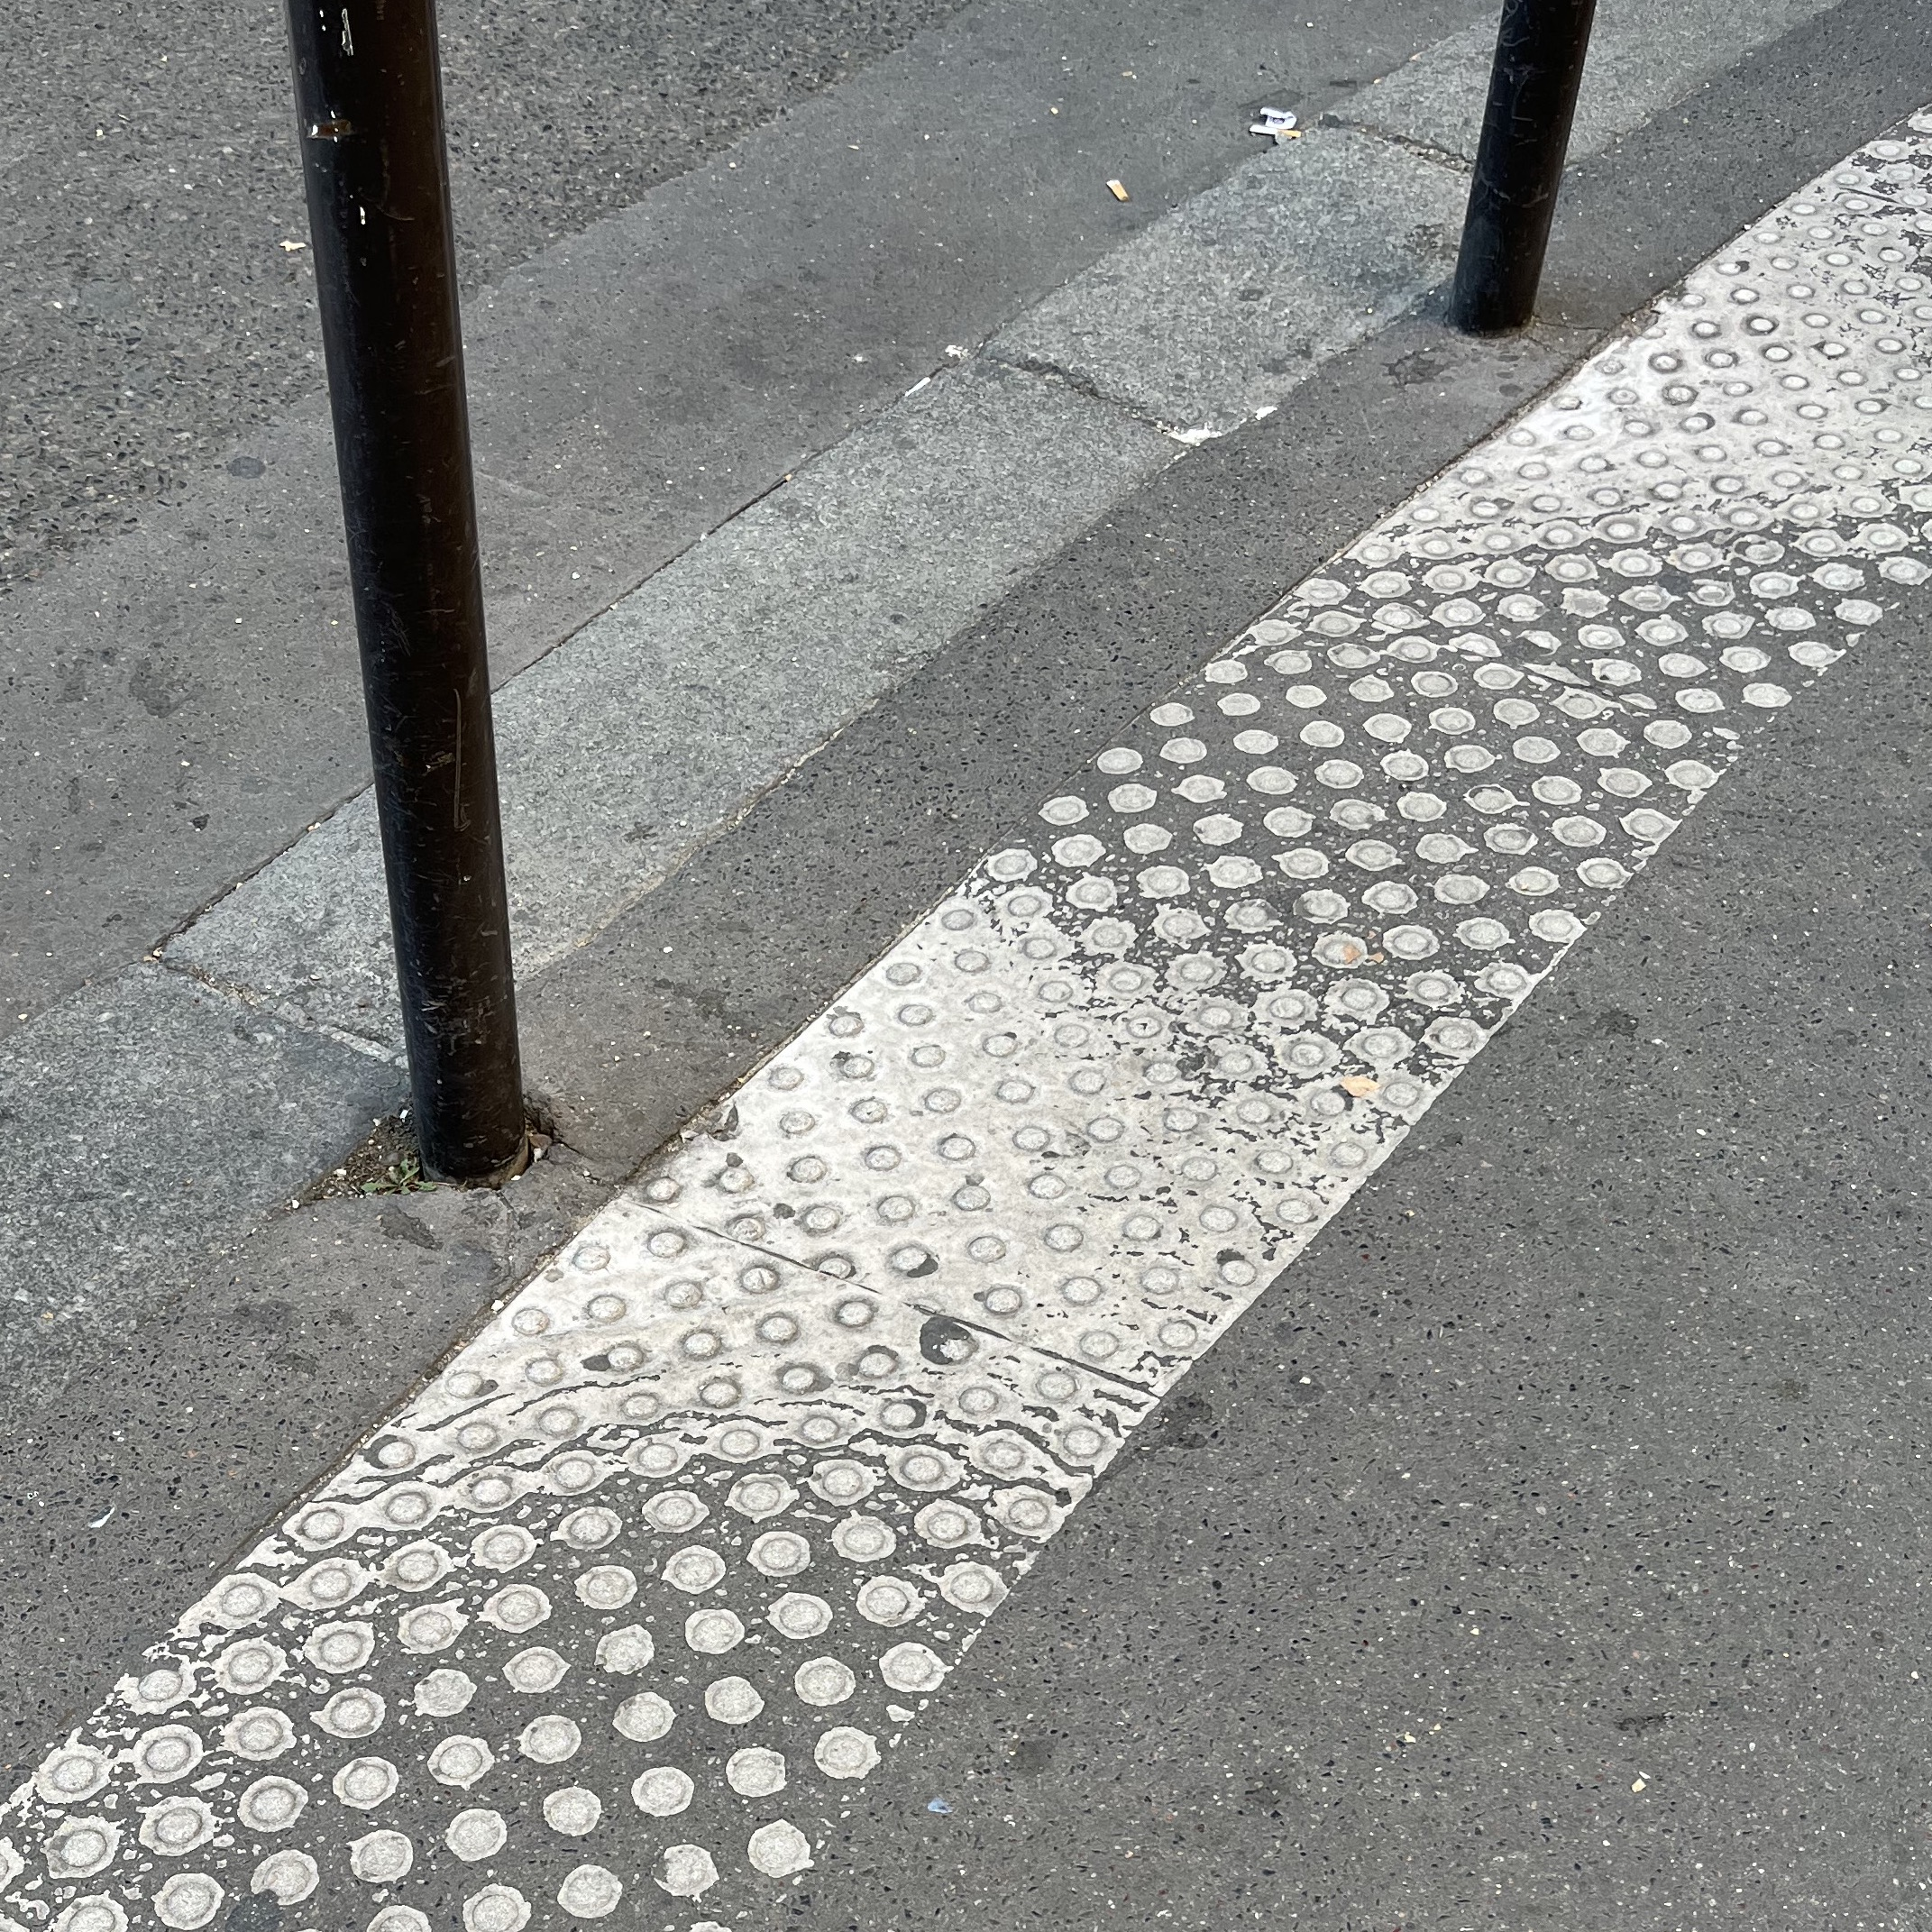
\includegraphics{images/modelisation/mod_bev.jpeg}} & Une \gls{bev} permet de détecter au pied ou à la canne la présence d'un passage piéton. On remarque sur l'image ci-contre qu'elle est abîmée, ce qui peut altérer sa détectabilité.\tabularnewline
        \resizebox{2cm}{!}{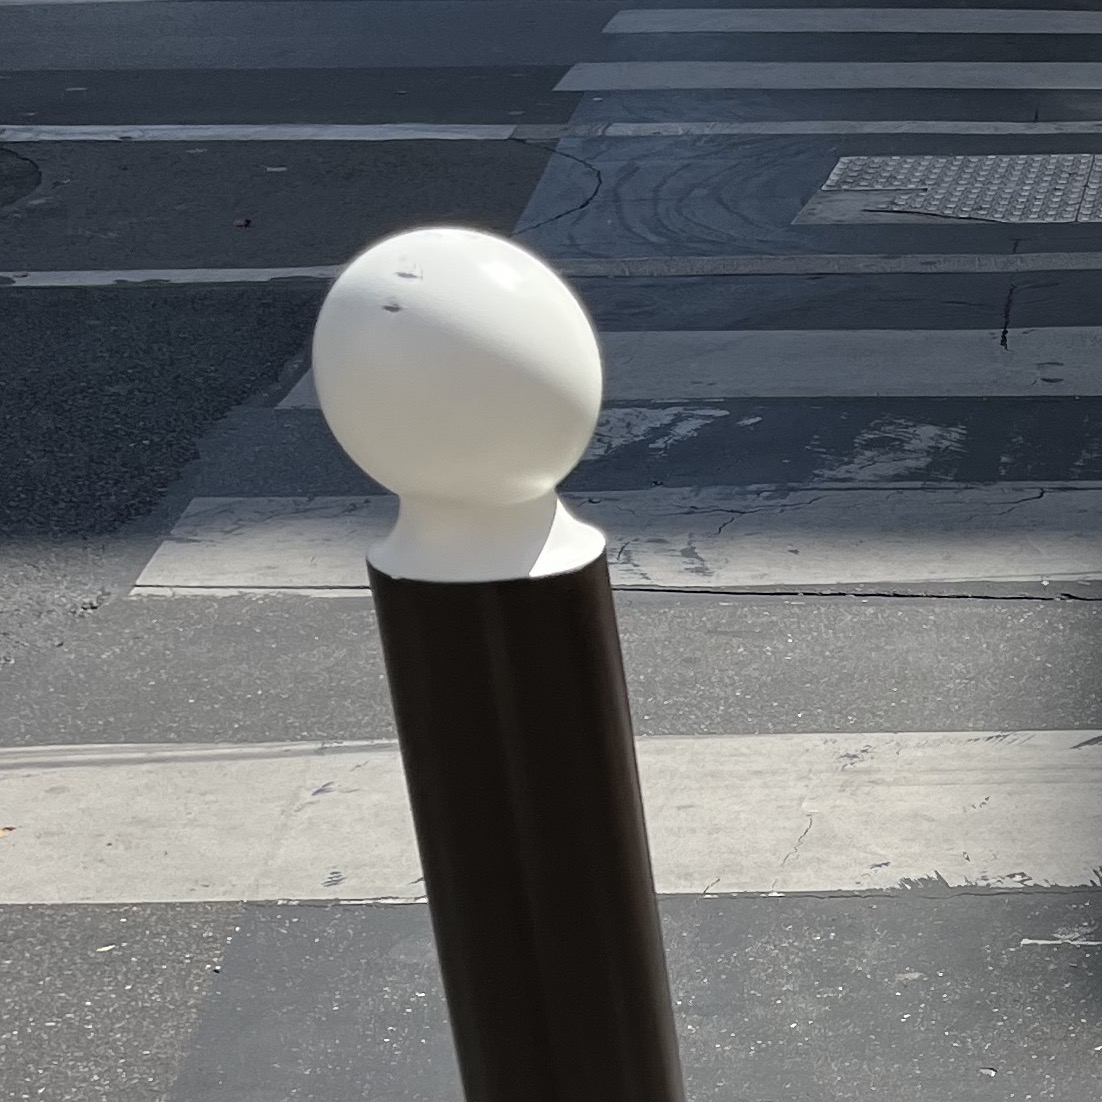
\includegraphics{images/modelisation/mod_poteau.jpeg}} & Les pôteaux parfois présents aux abords des passages piétons permettent à l'inster des \gls{bev} de signaler leur présence. Leur sommet est contrasté avec le corps pour permettre à une personne malvoyante de les distinguer.\tabularnewline
        \resizebox{2cm}{!}{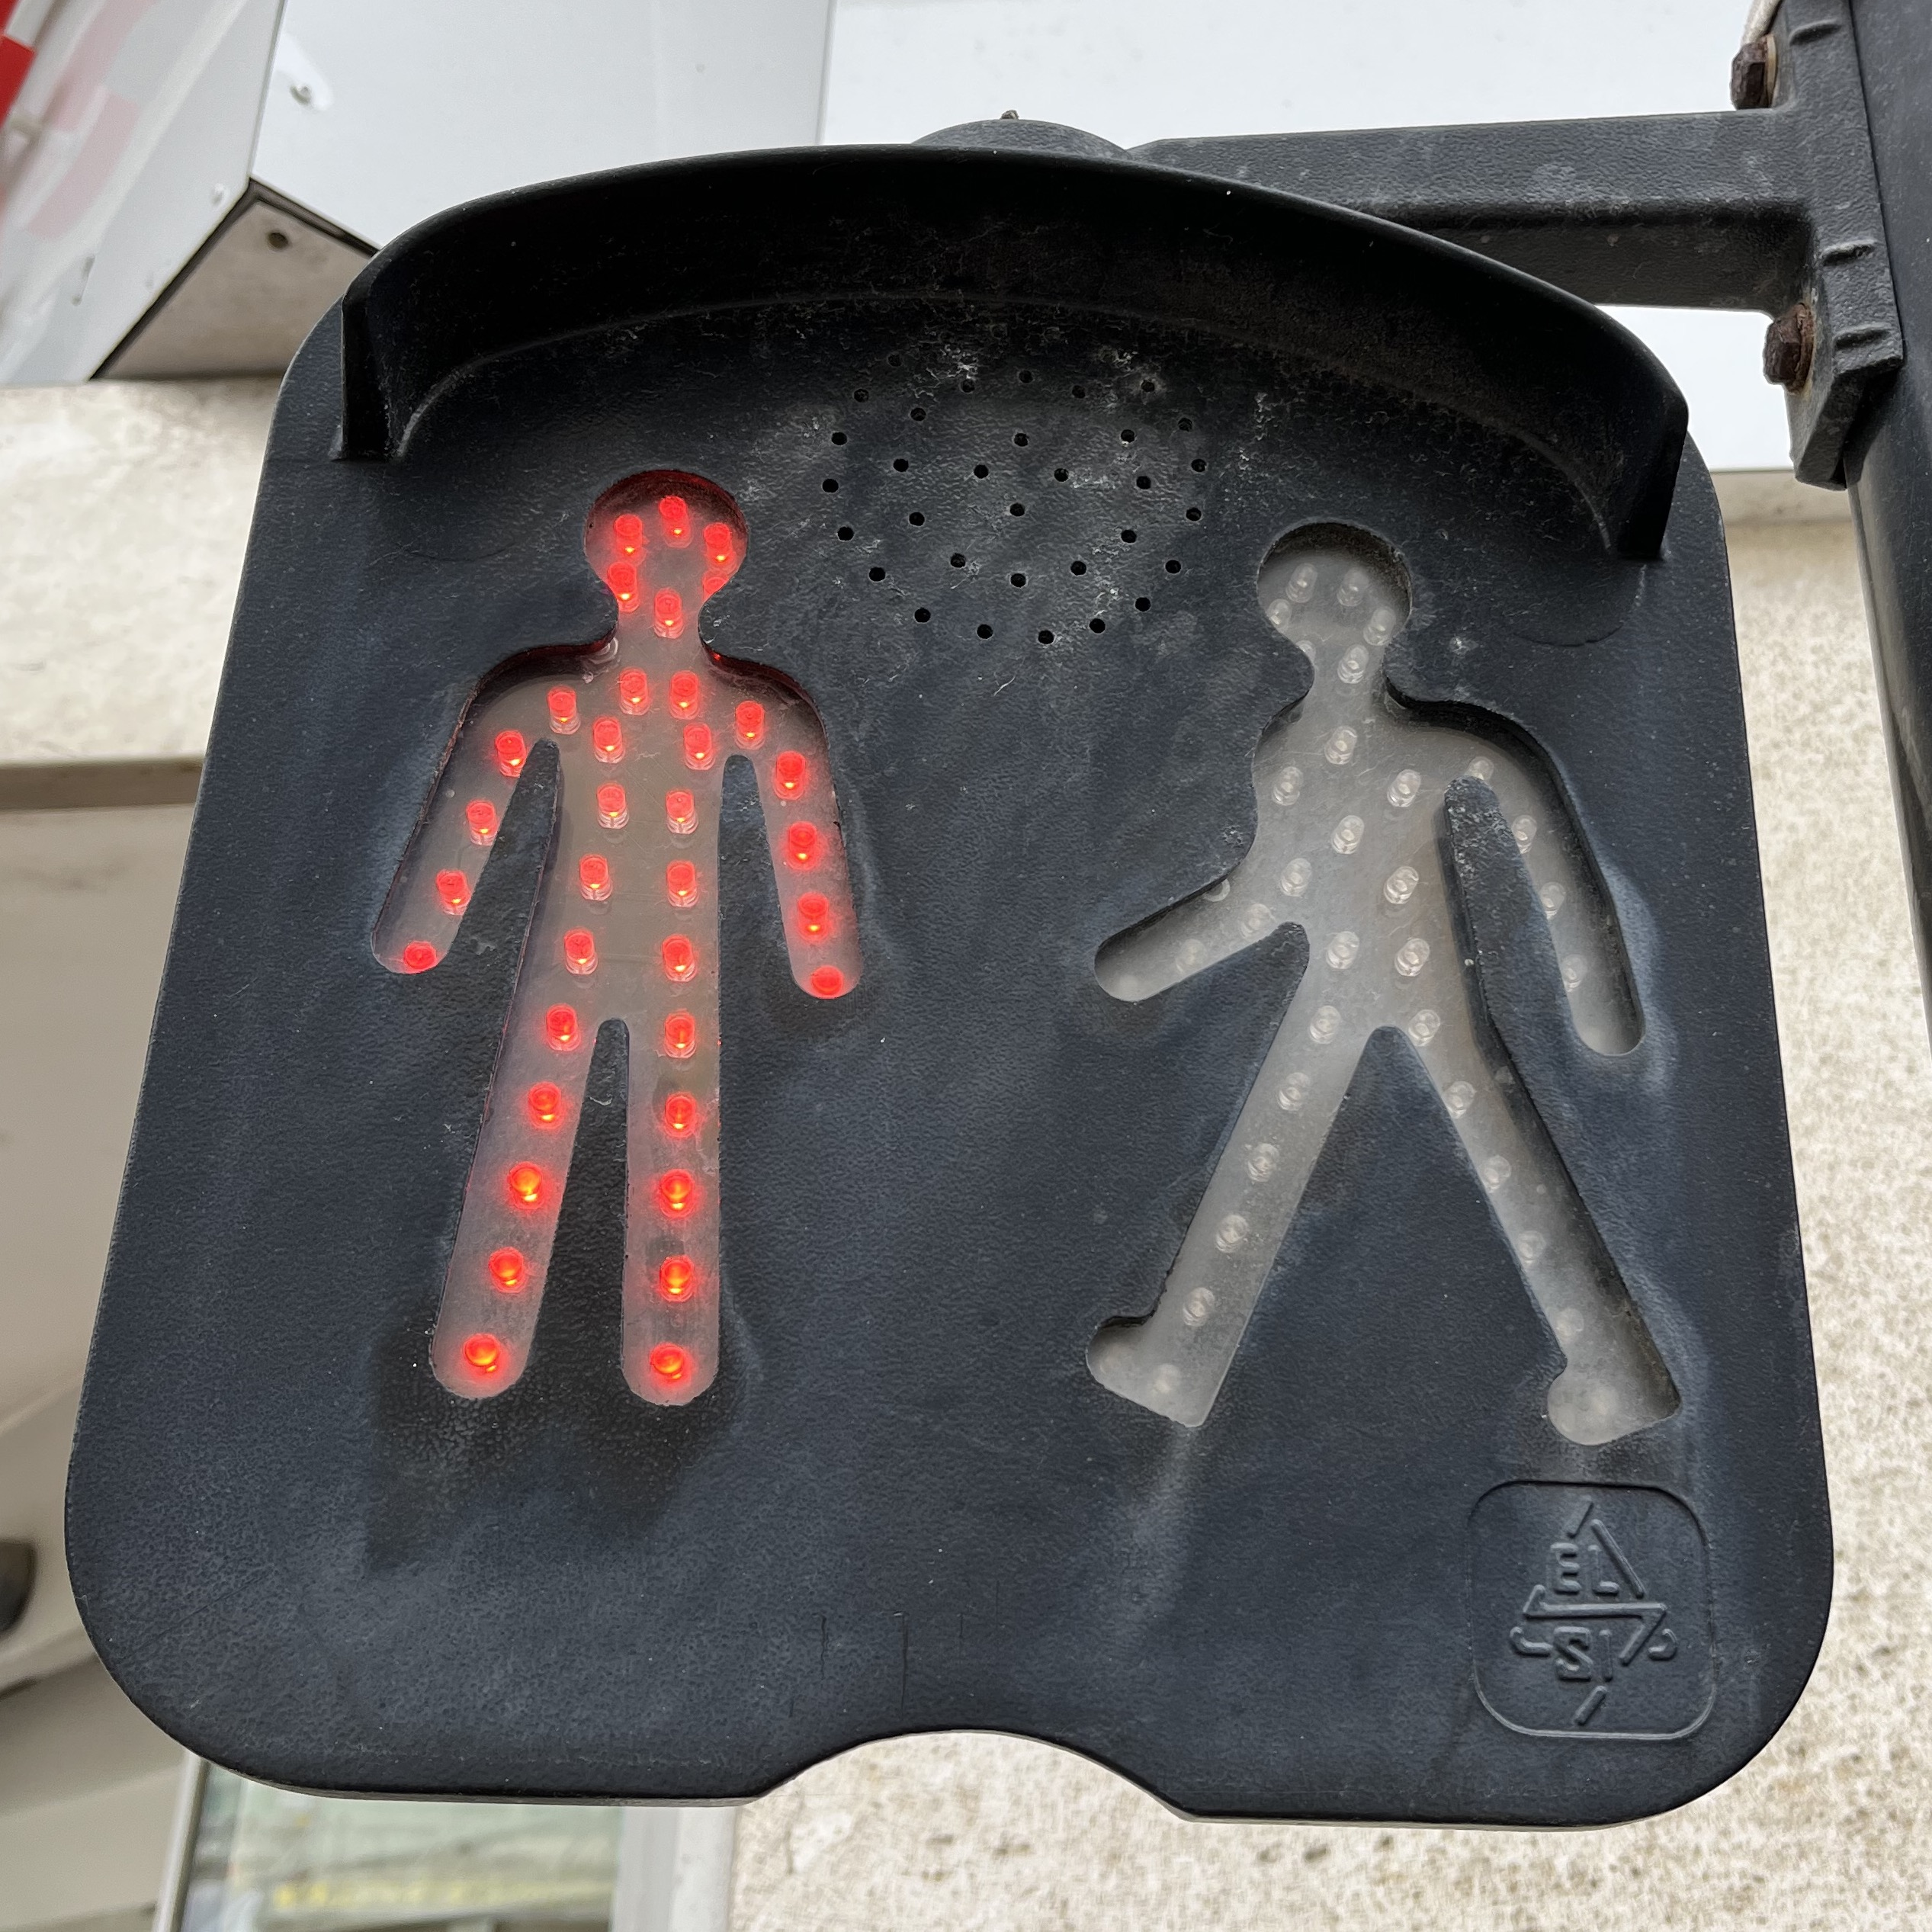
\includegraphics{images/modelisation/mod_feu_pieton.jpeg}} & Les feux de signalisation piéton peuvent être équipés d'une balise sonore. Le message joué par celle-ci varie, mais peut indiquer le nom de la rue traversée lorsque le feu est rouge. Un son de cloche est émis lorsque le feu est vert.\tabularnewline
    \end{tabular}
    \end{center}
    \caption{Équipements d'accessibilité au sein du carrefour.}
    \label{tab:modelisation_objets}
\end{table}

Au-delà des équipements d'accessibilité, le cycle des feux est également utile aux \glspl{pcdv} pour analyser la circulation et traverser en sécurité \cite{ratelle_manuel_2019}. Le cycle des feux correspond aux états successifs de chaque feu et permet de savoir quelles voies sont actuellement passantes. Il existe des modèles permettant la représentation de cette donnée, notamment au sein des outils de simulation de traffic routier \cite{Lopez2018}. Cependant, il n'existe actuellement aucun territoire la rendant accessible au sein d'une source de données ouverte.

\section{La modélisation d’un carrefour au sein d’OpenStreetMap}

\label{sec:modelisation_osm}

% La délimitation des carrefours n'existe pas dans OSM.
% Celle des branches non-plus.

\gls{osm} est une base de données géographique libre sous licence ODbL. Une de ses spécificités concerne son ouverture aux contributions après inscription, la carte étant intégralement réalisée par les utilisateurs. Nous verrons dans cette partie que, si elle n'est pas particulièrement spécialisée pour la modélisation des carrefours, ses capacités de représentation et la couverture spatiale et sémantique actuelle de certaines données la rendent intéressante pour notre cas d'utilisation.

\subsection{Une forte capacité de représentation}

Plus qu'une base de données géographique, \gls{osm} est une base de données topologique pouvant être représentée sous la forme d'un graphe non-connexe. 3 types d'objets peuvent être manipulés pour cartographier une entité : les points (node), les lignes (way), et les relations, chacun pouvant contenir une sémantique sous la forme de clés et de valeurs associées (voir Figure \ref{fig:mod_ex_donnee_osm})

% Illustration qui représente une ligne de bus, composée de ways aggrégées au sein d'une relation.
\begin{figure}
    \centering
    
\includegraphics{images/placeholder.jpg}
    \caption{Les différents objets d'\gls{osm} peuvent chacun contenir des attributs.}
    \label{fig:mod_ex_donnee_osm}
\end{figure}

% L'accessibilité piétonne dans OSM

OpenStreetMap est très souple concernant la représentation de l'accessibilité piétonne, et permet de cartographier finement de nombreux aménagements. Il est ainsi possible de représenter un graphe piéton contenant sous forme linéaire les trottoirs et les passages piétons. Au-delà de la géométrie, la sémantique associée permet de compléter les informations liées à l'accessibilité. Sur un passage piéton, cela peut permettre d'indiquer la présence de \glspl{bev} (\osmkey{tactile\_paving}), d'un feu piéton (\osmvalue{traffic\_signals} pouvant être associée à plusieurs clés), et de préciser si ce dernier est sonorisé (\osmkey{traffic\_signals:sound}). On peut également faire figurer la bordure du trottoir (\osmkey{kerb}) et son élévation par rapport à la chaussée.

\begin{figure}
    \centering
    \resizebox{15cm}{!}{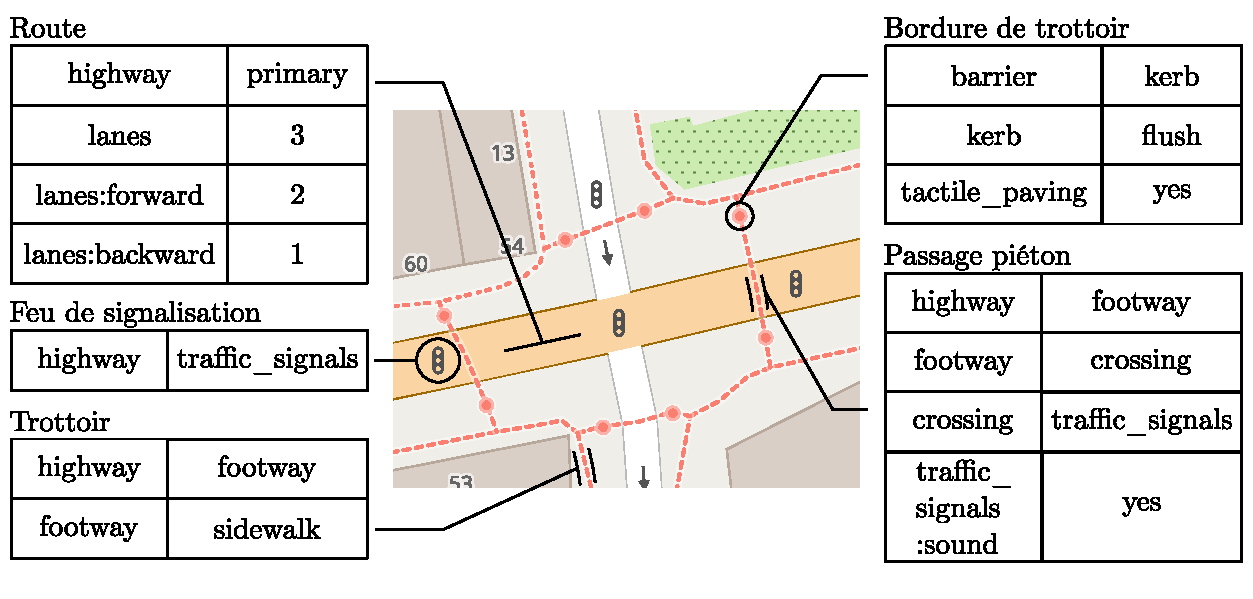
\includegraphics{images/modelisation/mod_anatomie_carrefour_osm.pdf}}
    \caption[Anatomie d'un carrefour dans OSM.]{Exemple de carrefour et des attributs associés dans OpenStreetMap. Outre le graphe piéton, des indications sur l'équipement d'accessibilité ou la largeur des voies (lanes) sont également présentes. Source : Contributeurs OpenStreetMap.}
    \label{fig:modelisation_anatomie_carrefour_osm}
\end{figure}

Au-delà de l'accessibilité de la voirie, la sémantique permet également de préciser l'accessibilité d'autres équipements. Cela vaut pour les bâtiments et commerces pour lesquels il est possible d'évaluer l'accessibilité d'une entrée (\osmkey{entrance}) en fauteuil roulant (\osmkey{wheelchair}) ainsi que la largeur de passage, mais également les aménagements tels que les arrêts de bus (\osmkey{highway}=\osmvalue{bus\_stop}) qui peuvent être abrités (\osmkey{shelter}) ou disposer d'un banc (\osmkey{bench}).

\newpar{}

% L'évolution de la sémantique sur OSM

Les clés et valeurs que nous évoquons se reposent sur la documentation établie par la communauté au sein du wiki d'\gls{osm}\footnote{https://wiki.openstreetmap.org/}. Si certaines clés et valeurs se sont imposées par l'usage (dit "de fait"\footnote{https://wiki.openstreetmap.org/wiki/Category:Key\_descriptions\_with\_status\_\%22de\_facto\%22}), la pratique usuelle pour faire évoluer la sémantique consiste à soumettre au vote de la communauté via le wiki une proposition de clés et valeurs supplémentaires pour représenter une nouvelle entité ou modifier un standard actuellement en vigueur. Nous pouvons illustrer cette pratique avec une donnée utile pour un piéton déficient visuel: le cycle des feux (evoqué en partie \ref{sec:mod_repere_carrefour}). S'il n'est pas possible avec la sémantique actuelle de représenter le cycle des feux sur \gls{osm}, un utilisateur propose en 2017 d'introduire une relation \osmkey{type}=\osmvalue{timing} \footnote{https://wiki.openstreetmap.org/wiki/Proposal:Traffic\_Signal\_Timings} pour modéliser cette information. Elle n'est pas, à l'heure actuelle, validée par la communauté car potentiellement inapplicables sur plusieurs territoires.

\newpar{}

% Ce que ne permet pas OpenStreetMap

La représentation des carrefours sur OpenStreetMap est en partie possible, mais ne correspond pas entièrement à notre besoin. Il existe la clé \osmkey{junction}, qui permet de pointer un carrefour voire de le délimiter (Figure \ref{fig:modelisation_carrefours_osm_paris}). Elle permet, au-delà de la valeur \osmvalue{yes} qui signifie que l'objet concerné est un carrefour, d'indiquer certains types de carrefour, en particulier les ronds-points avec la valeur \osmvalue{roundabout}\footnote{https://wiki.openstreetmap.org/wiki/Key:junction}. Cependant, la sémantique actuelle ne permet pas de modéliser les branches associées au carrefour. Par ailleurs, la plupart des carrefours ne sont pas représentés de cette manière. Un exemple de cartographie de carrefour dans \gls{osm} est présenté en figure \ref{fig:modelisation_anatomie_carrefour_osm}.

\begin{figure}
    \centering
    \resizebox{15cm}{!}{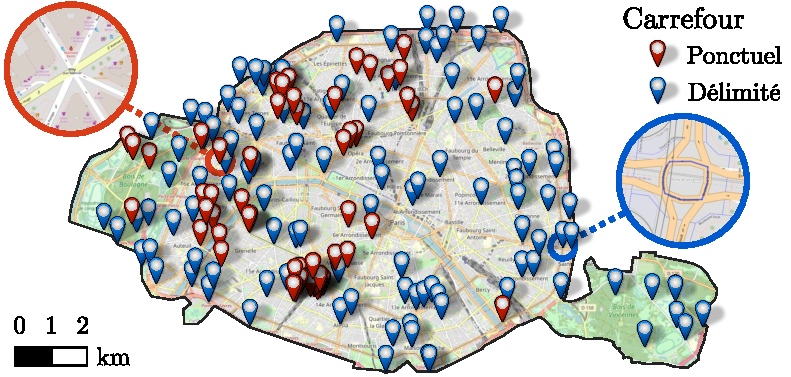
\includegraphics{images/modelisation/mod_carrefours_osm_paris.pdf}}
    \caption[Les carrefours OSM à Paris.]{À Paris, bien qu'il y ait beaucoup d'objets portant la clé \osmkey{junction}, la majorité des carrefours ne sont pas représentés sous cette forme. Source : Contributeurs OpenStreetMap.}
    \label{fig:modelisation_carrefours_osm_paris}
\end{figure}

\subsection{Des variations dans les modélisations}

\label{sec:modelisation_variation_pieton_osm}

% Variation dans la modélisation des trottoirs
% Variation dans la modélisation d'un passage piéton
% Etc.

Pour un même objet, plusieurs modélisations sont possibles voire peuvent coexister au sein d'\gls{osm}. Cela peut provenir d'une évolution de la sémantique (le modèle de description des transports en communs a évolué dans le temps), mais aussi de la possibilité d'avoir plusieurs niveaux de détails. Ce second cas s'illustre particulièrement bien sur l'accessibilité piétonne.

\newpar{}

Les trottoirs peuvent être représentés de trois manières différentes: sous une forme sémantique sur le filaire automobile, sous la forme d'un filaire séparé de la route, mais également sous la forme d'un polygone. Cette modélisation guidera également celle des passages piétons qui pourront être représentés comme un nœud sur le filaire automobile, potentiellement complété d'un filaire. Ces différentes modélisations sont illustrées en figure \ref{fig:modelisation_trottoir_osm}.

\begin{figure}
    \centering
    \begin{subfigure}[t]{.32\linewidth}
        \resizebox{4.5cm}{!}{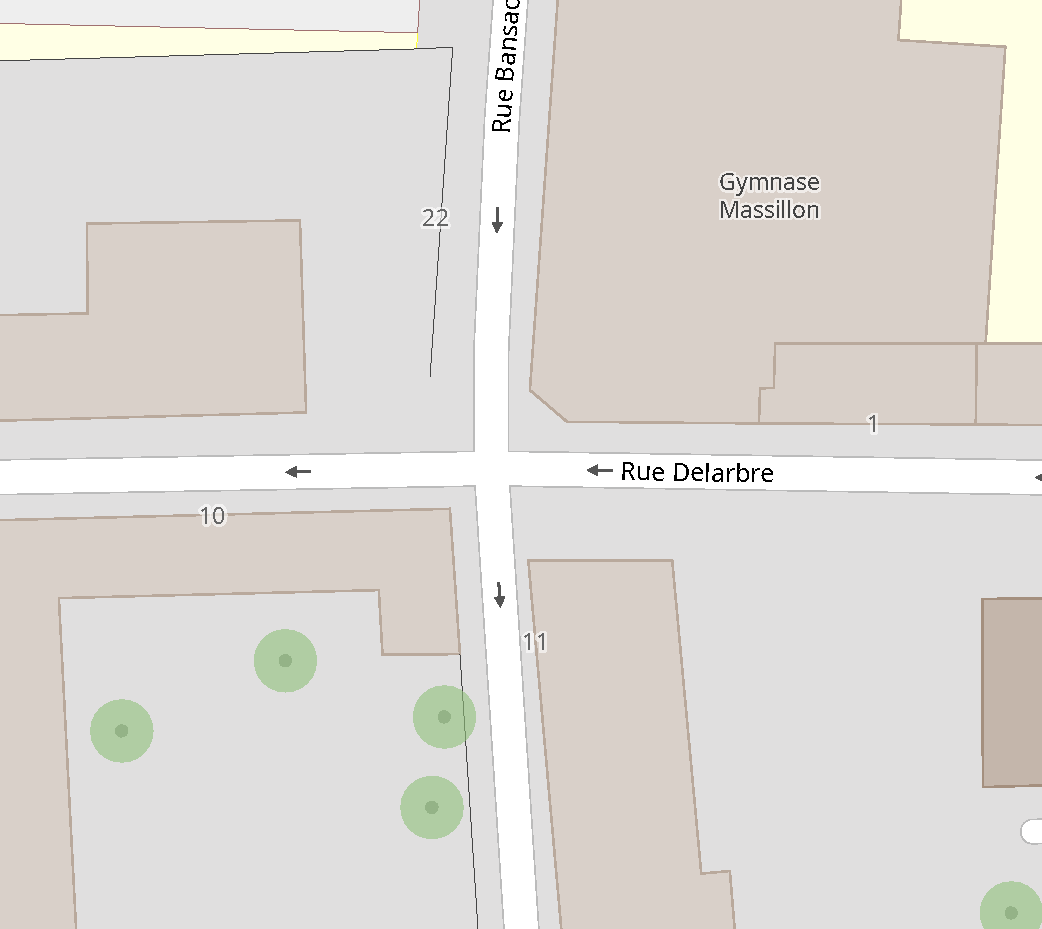
\includegraphics{images/modelisation/sw_semantic.pdf}}
        \caption{Les trottoirs sont ici présents sur les attributs \osmkey{sidewalk} de la route.}
    \end{subfigure}
    \begin{subfigure}[t]{.32\linewidth}
        \resizebox{4.5cm}{!}{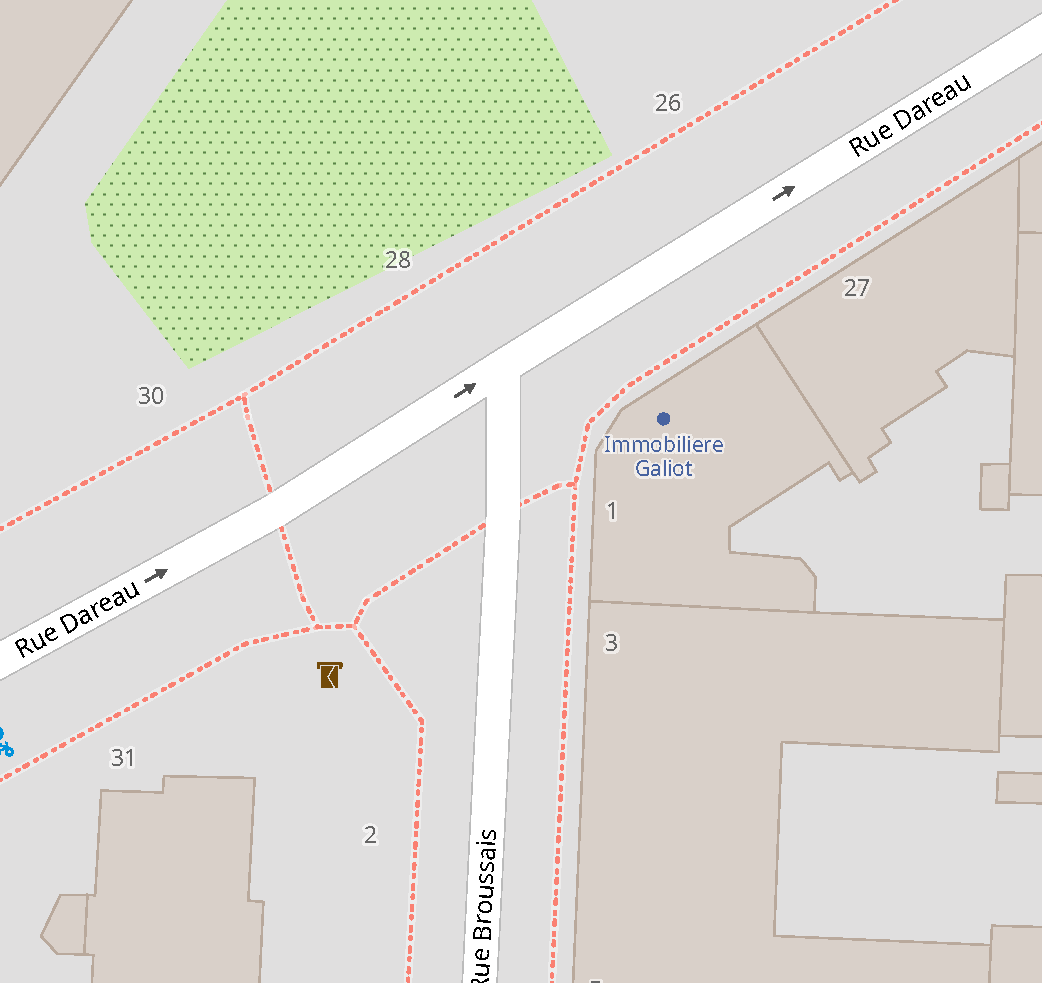
\includegraphics{images/modelisation/sw_line.pdf}}
        \caption{Les trottoirs sont tracés parallèlement à la route et portent la valeur \osmkey{footway}=\osmvalue{sidewalk}.}
    \end{subfigure}
    \begin{subfigure}[t]{.32\linewidth}
        \resizebox{4.5cm}{!}{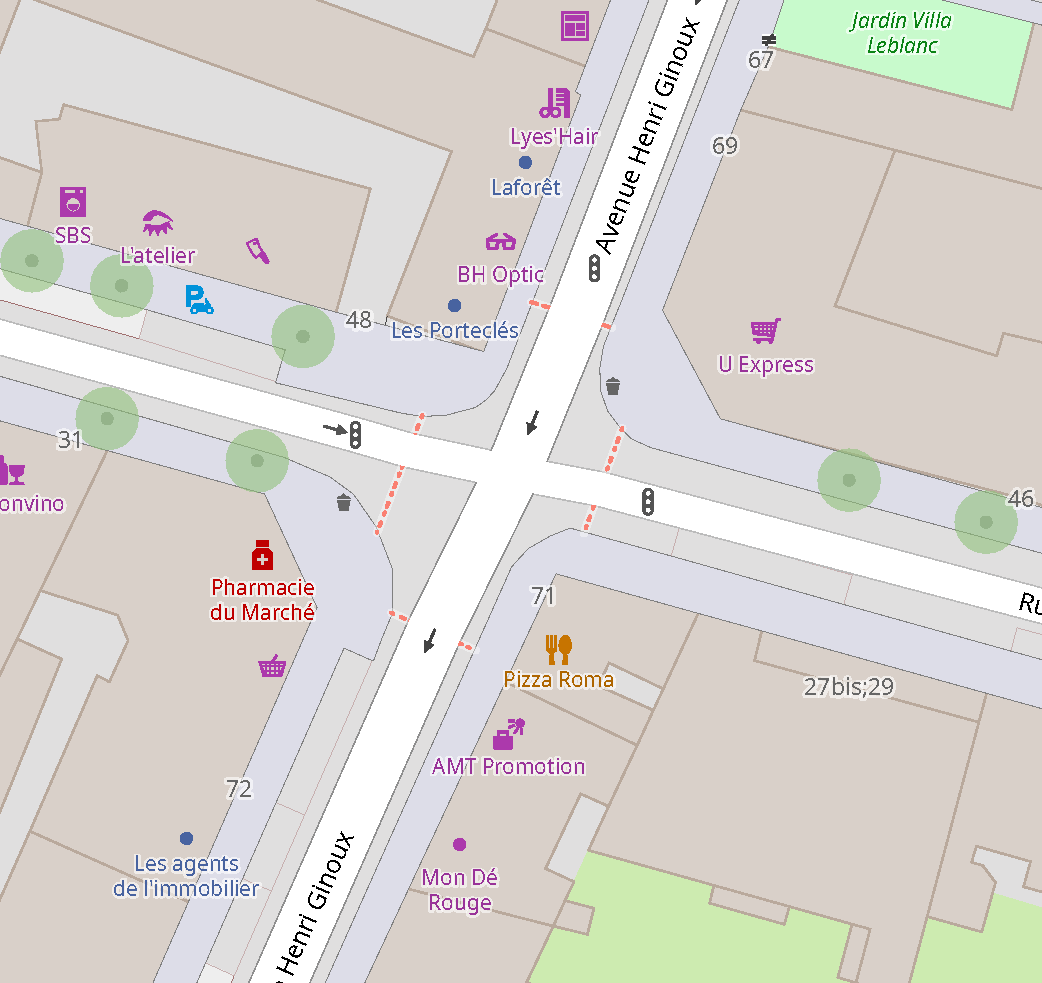
\includegraphics{images/modelisation/sw_polygon.pdf}}
        \caption{Les trottoirs sont tracés en surfaces. Ils contiennent les mêmes valeurs que les trottoirs linéaire, complétés de \osmvalue{area}=\osmvalue{yes}}
    \end{subfigure}
    \caption{Illustration des différentes modélisations de trottoirs possibles sur \gls{osm}. Source: Contributeurs OpenStreetMap.}
    \label{fig:modelisation_trottoir_osm}
\end{figure}

\newpar{}

% L'évolution du filaire piéton au sein d'\gls{osm}.

Par ailleurs, les pratiques sont localement variées. Le journal d'un utilisateur d'OpenStreetMap\footnote{\url{https://www.openstreetmap.org/user/Hungerburg/diary/395540}} présente l'historique de cartographie des trottoirs jusqu'à 2021 en comparant l'évolution des trottoirs cartographiés en sémantique sur la route et les trottoirs filaires sur la Grande-Bretagne et la Pologne (voir figure \ref{fig:modelisation_osm_gb_pologne}). On note dans tous les cas une évolution significative de l'intérêt pour cette thématique au fil du temps.

\begin{figure}
    \centering
    \begin{subfigure}[t]{.49\linewidth}
        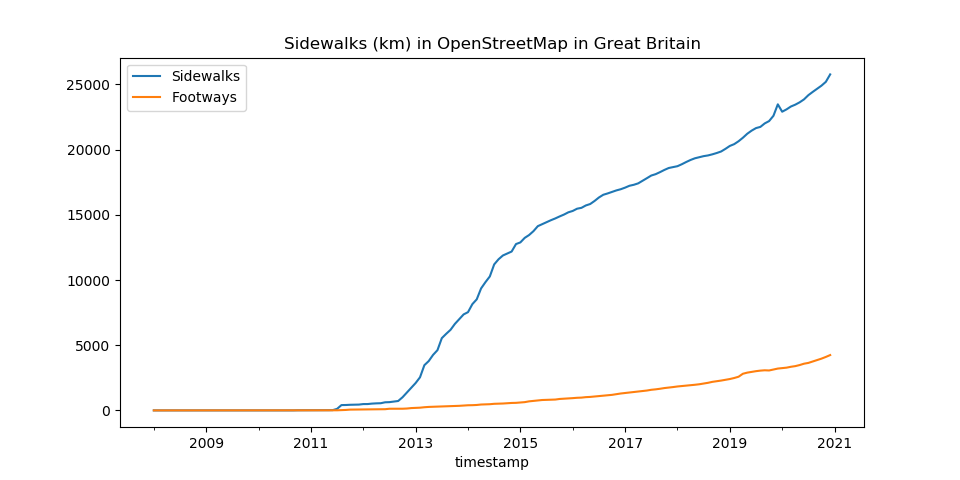
\includegraphics[width=\textwidth]{images/modelisation/Sidewalks-Length-Britain.png}
        \caption{Évolution de la cartographie des trottoirs en Grande-Bretagne.\label{fig:modelisation_osm_gb}}
    \end{subfigure}
    \begin{subfigure}[t]{.49\linewidth}
        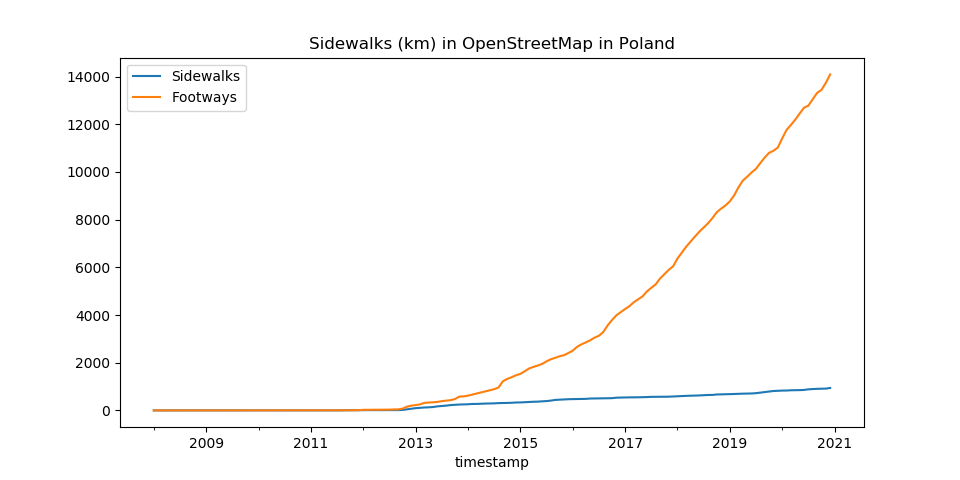
\includegraphics[width=\textwidth]{images/modelisation/Sidewalks-Length-Poland.png}
        \caption{Évolution de la cartographie des trottoirs en Pologne. \label{fig:modelisation_osm_pologne}}
    \end{subfigure}
    \caption{Les pratiques de cartographies peuvent être localisées sur OSM. En Pologne, le filaire piéton s'est majoritairement développé au contraire de la Grande-Bretagne où il reste majoritairement présent en sémantique du réseau routier. Source: \url{https://www.openstreetmap.org/user/Hungerburg/diary/395540}.}
    \label{fig:modelisation_osm_gb_pologne}
\end{figure}

\section{Un modèle de carrefour}

Pour utiliser la donnée \gls{osm} dans un contexte spécifique, il est préconisé de la manipuler à l'aide d'un modèle de donnée spécialisé intermédiaire \cite{Touya2014}. Nous proposons dans un premier temps une modélisation objet générique de la donnée \gls{osm}, que nous appliquons dans un second temps à la modélisation du carrefour. Enfin, nous présentons les méthodes permettant d'instancier ce modèle depuis OpenStreetMap.

\subsection{OSM-Objet : une modélisation objet de la donnée OpenStreetMap}

\begin{figure}
\centering
\begin{plantuml}

    @startuml
    object Node {
        int id
        float x
        float y
    }

    object AbstractNode

    object NodeDecorator

    object Crosswalk
    object TrafficLight

    Node -r-|> AbstractNode
    NodeDecorator -u-|> AbstractNode
    AbstractNode "1" -* "1" NodeDecorator
    Crosswalk -u-|> NodeDecorator
    TrafficLight -u-|> NodeDecorator
    @enduml
    
\end{plantuml}
\caption[Modèle OSM-Objet.]{Modèle OSM-Objet. Les classes Crosswalk et TrafficLight sont présentes pour illustrer l'utilisation.}
\label{fig:modelisation_osm_objet}
\end{figure}

Comme présenté dans la partie \ref{sec:modelisation_osm}, les objets représentés au sein d'\gls{osm} sont définis par un ensemble de clés et de valeurs. Ainsi, pour manipuler chaque objet, il est nécessaire de déterminer l'ensemble des clés et valeurs qui vont le définir. En ce sens, il est plus commode de manipuler un modèle intermédiaire pour lequel cet ensemble est prédéfini. Cette problématique a déjà été abordée au sein des ontologies réalisées autour d'\gls{osm}\cite{Codescu2011,Hombiat2017} ou des travaux qui s'appuient sur ces données \cite{Touya2014}. Cependant, une particularité des capacités sémantique d'OpenStreetMap est qu'il est possible que la somme des clés et des valeurs d'une entité corresponde à plusieurs objets dans la vie réelle. Un exemple typique concerne les passages piétons représentés par un nœud et dont la sémantique contient souvent à la fois celle associée au passage piéton, ainsi que celle associée au feu de circulation. Pour gérer cette particularité, nous proposons un modèle de données orienté objet appelé OSM-Objet.

\newpar{}

OSM-Objet se repose sur le patron de conception du décorateur \cite{Gamma1994a}. Le décorateur permet d'ajouter dynamiquement des fonctionnalités à un objet sans passer par une sous-classe, et en conservant la même interface pour le manipuler. Dans notre cas, comme l'illustre la figure \ref{fig:modelisation_osm_objet}, nous pouvons manipuler un nœud, qui peut être simultanément un passage piéton et un feu de signalisation.

\subsection{Application à la modélisation du carrefour}

\begin{figure}
    \centering
    \begin{plantuml}
        @startuml

        enum Direction {
            IN
            OUT
        }

        object Lane {
            int id
        }
        object Bus
        object Road

        object Way {
            int id
            string name
        }

        object Node {
            int id
            float x
            float y
        }
        object AbstractNode
        object NodeDecorator
        object TrafficLight
        object PedestrianTrafficLight
        object Crosswalk

        object Branch {
            int id
        }

        object Intersection

        object PedestrianNode {
            int id
        }
        object Sidewalk
        object Island
        object Crossing

        'Relations

        'Decorator part
        Node -r-|> AbstractNode
        NodeDecorator -l-|> AbstractNode
        AbstractNode "1" -r-* "1" NodeDecorator
        TrafficLight -u-|> NodeDecorator
        PedestrianTrafficLight -u-|> NodeDecorator
        Crosswalk -u-|> NodeDecorator

        'Way part
        Way "*" o-r- "2" Node

        'Lanes part
        Way "1" *-u- "*" Lane
        Lane <|-r- Bus
        Lane <|-r- Road
        Lane o-l- Direction

        'Branch part
        Branch "1" o-r- "*" Way
        Intersection "1" *-r- "*" Branch
        Branch "1" *-d- "1" Crossing

        'Pedestrian node part
        Way "*" o-d- "0..2" PedestrianNode
        Sidewalk -r-|> PedestrianNode
        Island -l-|> PedestrianNode
        PedestrianNode "2" -d-o "*" Crosswalk

        'Crossing part
        Crossing o-r- Crosswalk

        'Placement commands
        PedestrianTrafficLight -d[hidden]- TrafficLight
        Crosswalk -u[hidden]- PedestrianTrafficLight

        @enduml 
    \end{plantuml}
    \caption[Modèle CrModel.]{Modèle CrModel architecturé autour d'OSM-Objet.}
    \label{fig:modelisation_crmodel}
\end{figure}

Pour modéliser le carrefour, nous proposons CrModel, le modèle de données en figure \ref{fig:modelisation_crmodel}. Il représente un graphe du carrefour, dont la classe Node figure les nœuds et la classe Way figure les tronçons. Nous avons architecturé les nœuds autour d'OSM-Objet. Chaque branche (Branch) est identifiée par un numéro et contient tous les tronçons qui en font partie. Une  branche peut également contenir une traversée (Crossing). Nous avons également introduit certains comportements spécifiques:

\begin{itemize}
    \item Les différentes voies d'une route sont identifiées par des attributs sur \gls{osm}. Nous avons donc ajouté la classe Lane pour représenter cette information dans un paradigme objet.
    \item Les trottoirs (Sidewalk) et les îlots (Island) sont également des classes indépendantes et non de la sémantique sur les tronçons. Chaque tronçon peut contenir deux PedestrianNode, permettant d'indiquer quel trottoir ou îlot est à sa droite ou à sa gauche.
    \item Nous voulons pouvoir indiquer pour chaque branche si et comment elle se traverse. Pour cela, nous avons introduit la classe Crossing qui consiste en une séquence de passages piétons entre deux trottoirs. Les passages piétons eux-même sont composés de deux PedestrianNode qui indiquent où se situe le passage piéton (entre un trottoir et îlot par exemple).
\end{itemize}

\newpar{}

Pour instancier CrModel, il est nécessaire de disposer d'un graphe routier dont la sémantique identifie les branches, la position des trottoirs et des îlots, et les passages piétons. Les parties suivantes de ce chapitre détaillent:
\begin{itemize}
    \item le processus de segmentation des carrefours au sein d'un graphe routier issu d'\gls{osm},
    \item le processus qui, à partir de la segmentation, dérive les informations piétonnes du carrefour: trottoirs, îlots, traversées.
\end{itemize}

\section{Segmenter un carrefour dans le graphe d'\gls{osm}}

Du point de vue d'un piéton, la bordure entre le cœur de carrefour et les branches (voir définition \ref{def:modelisation_couverture_routiere_complète}) sera généralement située au niveau des passages piétons pour chaque branche du carrefour. Si une branche n'a pas de passage piéton, cette séparation sera située là où les véhicules s'arrêtent (feu de circulation, panneau stop, etc.) comme illustré à la figure \ref{fig:modelisation_limite_carrefourA}. En cas d'absence de toute signalisation, la limite sera placée aussi près que possible pour éviter d'étendre sa zone dans la branche adjacente, comme illustré à la figure \ref{fig:modelisation_limite_carrefourB}.

\newpar{}

Comme évoqué en partie \ref{sec:modelisation_variation_pieton_osm} l'infrastructure piétonne est aujourd'hui encore rarement modélisée séparément de la route. Par conséquent, nous proposons dans la suite de cette partie de considérer uniquement la donnée contenue par les nœuds et arêtes du réseau routier. Nous supposons que les informations suivantes (reconstruites ou directement disponibles) sont accessibles sur le réseau routier:
\begin{itemize}
    \item La largeur de la route, directement accessible (\osmkey{width}) ou estimée en fonction du type de route (\osmkey{highway}) et du nombre de voies (\osmkey{lanes}),
    \item le type de route, si elle correspond à un carrefour (\osmkey{junction} ou \osmkey{highway} = \osmvalue{*\_link}),
    \item le nom de la route (\osmkey{name}),
    \item le type du nœud s'il décrit un élément de l'infrastructure (clé \osmkey{highway}): passage piéton (\osmvalue{crossing}), feu de circulation (\osmvalue{traffic\_signal}), panneau stop (\osmvalue{stop}) ou cédez-le-passage (\osmvalue{give\_way}).
\end{itemize}

\newpar{}

Cette partie est issue de travaux réalisés en collaboration avec Jean-Marie Favreau et publiés dans \cite{Favreau2022} et \cite{Kalsron2022}.

\subsection{Étapes d'une segmentation multi-échelle de carrefour}

\begin{figure}
    \centering
    \begin{subfigure}[t]{.49\linewidth}
        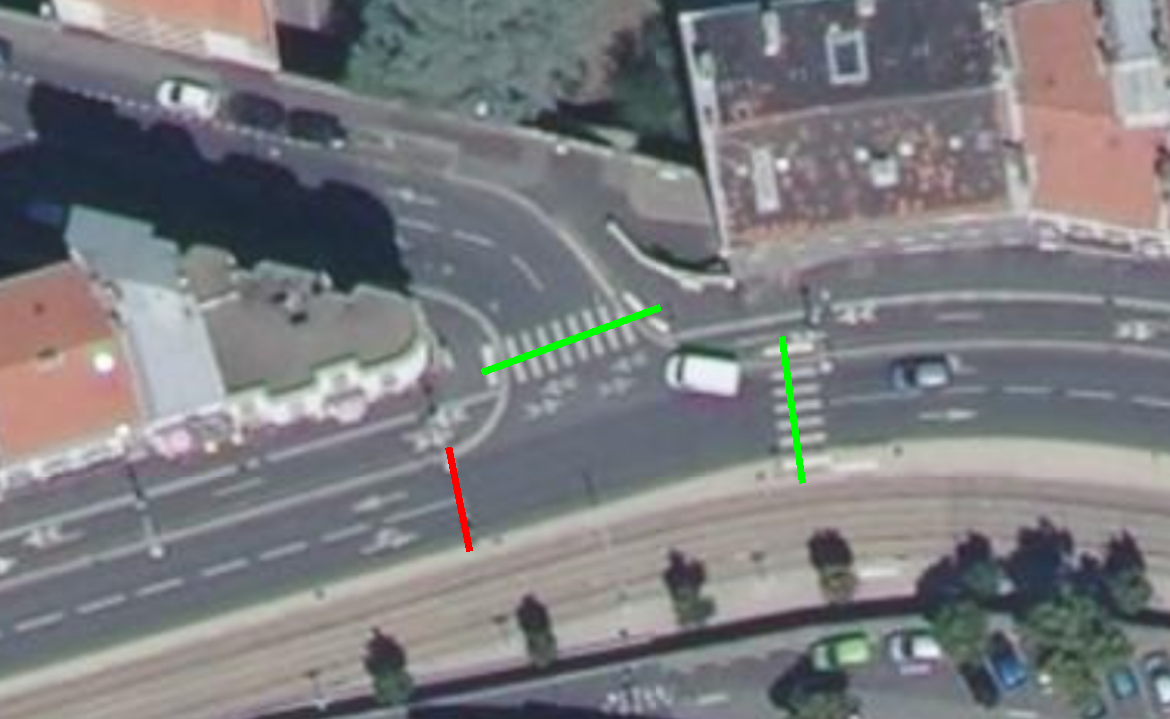
\includegraphics[width=\textwidth]{images/modelisation/segmentation/orthophoto-1.pdf}
        \caption{Un carrefour dont les bordures sont définies par deux passages piétons (lignes vertes) et un feu de signalisation (ligne rouge).\label{fig:modelisation_limite_carrefourA}}
    \end{subfigure}
    \begin{subfigure}[t]{.49\linewidth}
        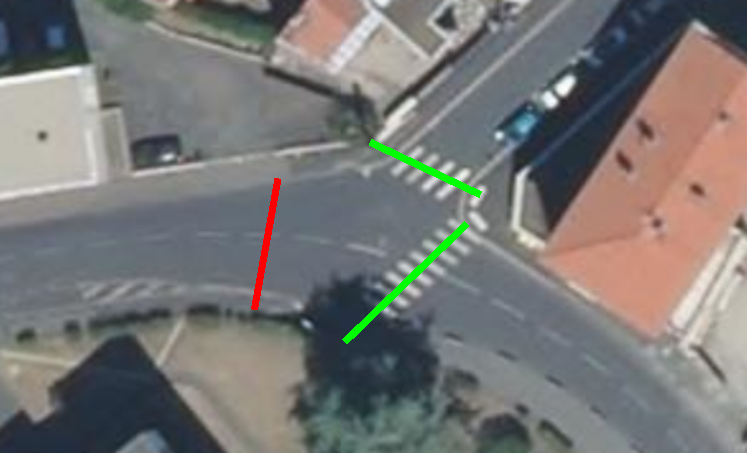
\includegraphics[width=\textwidth]{images/modelisation/segmentation/orthophoto-2.pdf}
        \caption{Un carrefour dont les bordures sont définies par deux passages piétons (lignes vertes) et une branche sans marquage (ligne rouge). \label{fig:modelisation_limite_carrefourB}}
    \end{subfigure}
    \caption{Les bordures des carrefours sont situées au niveau des infrastructures, si elles existent. Fond de plan: Géoportail © IGN. Source: \cite{Favreau2022}.}
    \label{fig:modelisation_limite_carrefour}
\end{figure}

\begin{figure}
    \centering
    \resizebox{15cm}{!}{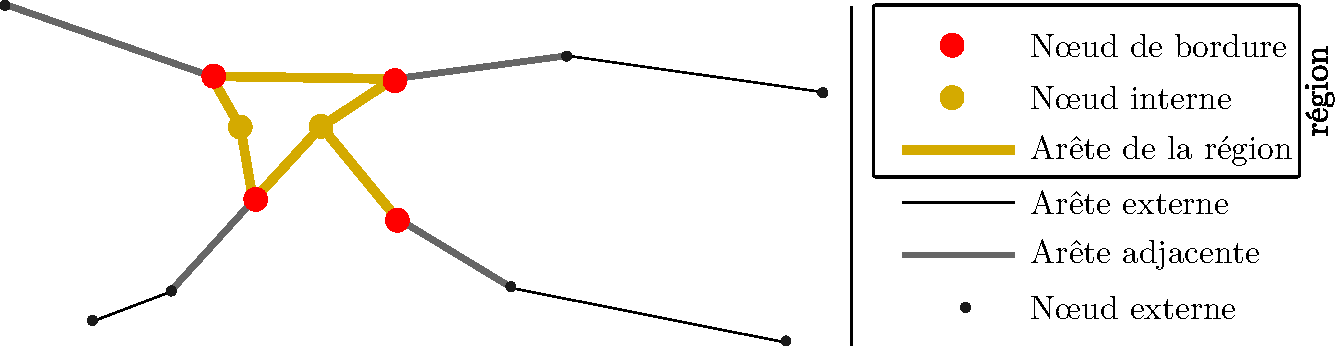
\includegraphics{images/modelisation/segmentation/region.pdf}}
    \caption{Exemple de région définie dans le graphe. Source: \cite{Favreau2022}.}
    \label{fig:modelisation_region_segmentation}
\end{figure}

On considère un graphe routier $G_r = (V_r,E_r)$ dont les nœuds et les arêtes contiennent des informations sémantiques sous la forme de clés-valeurs. Nous définission une segmentation du graphe routier en identifiant pour chaque région de la segmentation un ensemble non-vide de nœuds et un ensemble possiblement vide d'arêtes, avec la contrainte suivante : si une arête appartient à une région, ses deux nœuds lui appartiennent également.
Pour chaque région, nous identifions deux types de nœuds: les \textbf{nœuds internes} (uniquement connectés aux arêtes appartenant à la région), et les \textbf{nœuds de bordure} (connectés à au moins une arête appartenant à la région, et une arête n'appartenant pas à la région) (voir figure \ref{fig:modelisation_region_segmentation}).
Les \textbf{arêtes adjacentes} d'une région sont identifiées comme les arêtes qui n'appartiennent pas à la région, mais dont un une des extrêmités en fait partie.

\subsubsection{Carrefour élémentaire}

La première étape de la détection des carrefours que nous proposons consiste à évaluer pour chaque nœud la probabilité qu'il s'agisse d'un nœud interne ou d'un nœud de bordure d'un carrefour.
Cette première identification nous permet de caractériser:

\begin{itemize}
    \item Les passages piétons comme probables nœuds de bordure d'un carrefour
    \item Les nœuds représentant les entités de contrôle du traffic (feu de signalisation, panneaux stop et cédez-le-passage) comme possibles nœuds de bordure d'un carrefour
    \item Les nœuds avec une cardinalité supérieure à deux, et dont les arêtes adjacentes ont des noms de rue distincts, comme probablement nœuds internes d'un carrefour, et considérés comme nœuds graine dans les étapes suivantes de l'algorithme
\end{itemize}

\begin{figure}
    \centering
    \begin{subfigure}[t]{.49\linewidth}
        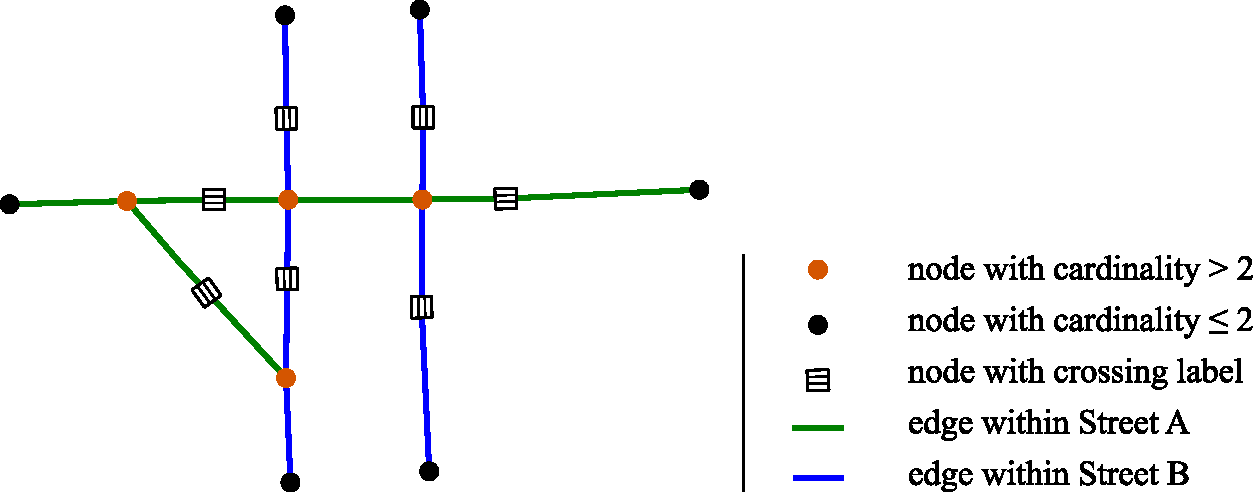
\includegraphics[width=\textwidth]{images/modelisation/segmentation/segmentation-step1.pdf}
        \caption{Un graphe labellisé tel qu'il peut être extrait d'\gls{osm}.\label{fig:modelisation_segmentation_step1}}
    \end{subfigure}
    \begin{subfigure}[t]{.49\linewidth}
        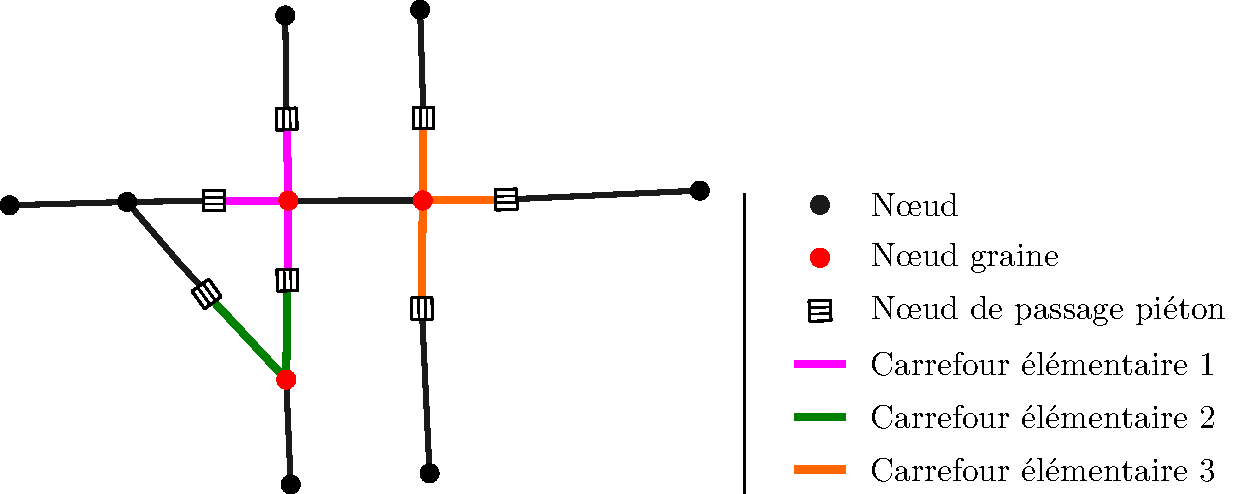
\includegraphics[width=\textwidth]{images/modelisation/segmentation/segmentation-step2.pdf}
        \caption{Carrefours élémentaires générés depuis le graphe de gauche. \label{fig:modelisation_segmentation_step2}}
    \end{subfigure}
    \caption{Résultat de la segmentation d'un carrefour élémentaire. Source: \cite{Favreau2022}.}
    \label{fig:modelisation_segmentation_step1&2}
\end{figure}

\subsubsection{Approche multi-échelle}

Cette première identification (voir figure \ref{fig:modelisation_segmentation_step1}) permet de construire les carrefours élémentaires, en utilisant la sémantique de la voie pour guider la décision d'étendre et consolider la segmentation de chaque nœud graine (voir figure \ref{fig:modelisation_segmentation_step2}). En revanche, elle ne correspond pas réellement à l'intuition d'un piéton. En effet, elle produit plusieurs petites régions souvent proches les unes des autres. Cependant, nous pouvons identifier ces dernières comme des sous-parties d'un carrefour plus complexe. En utilisant la sémantique, la géométrie et la topologie des arêtes adjacentes à chaque carrefour, nous proposons un algorithme pour assembler les carrefours élémentaires en carrefours fonctionnels.

\begin{figure}
    \centering
    \begin{subfigure}[t]{.49\linewidth}
        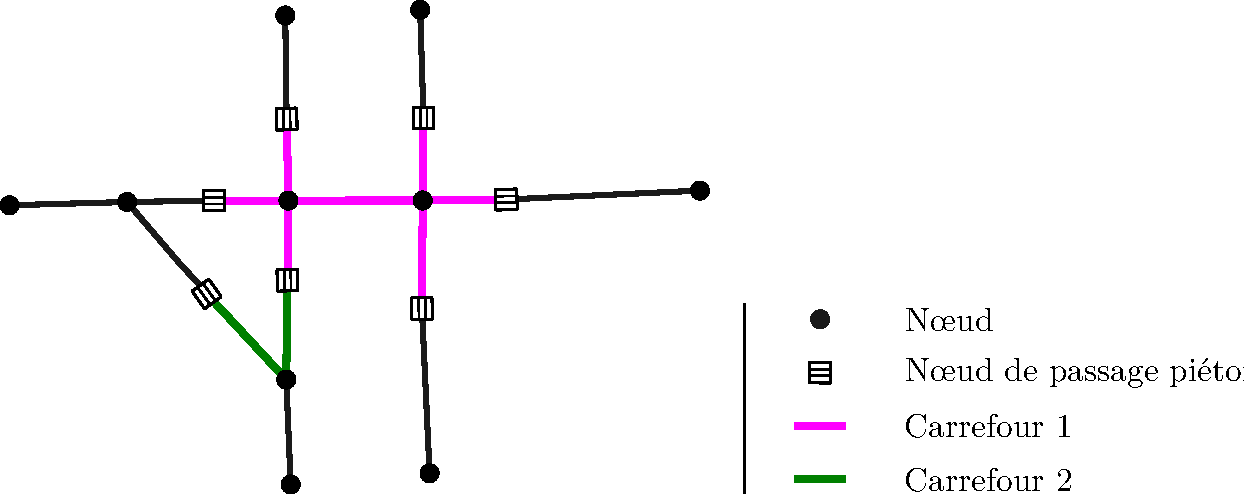
\includegraphics[width=\textwidth]{images/modelisation/segmentation/segmentation-step3.pdf}
        \caption{Résultat de la première étape d'assemblage des carrefours élémentaires de la figure \ref{fig:modelisation_segmentation_step2}.\label{fig:modelisation_segmentation_step3}}
    \end{subfigure}
    \begin{subfigure}[t]{.49\linewidth}
        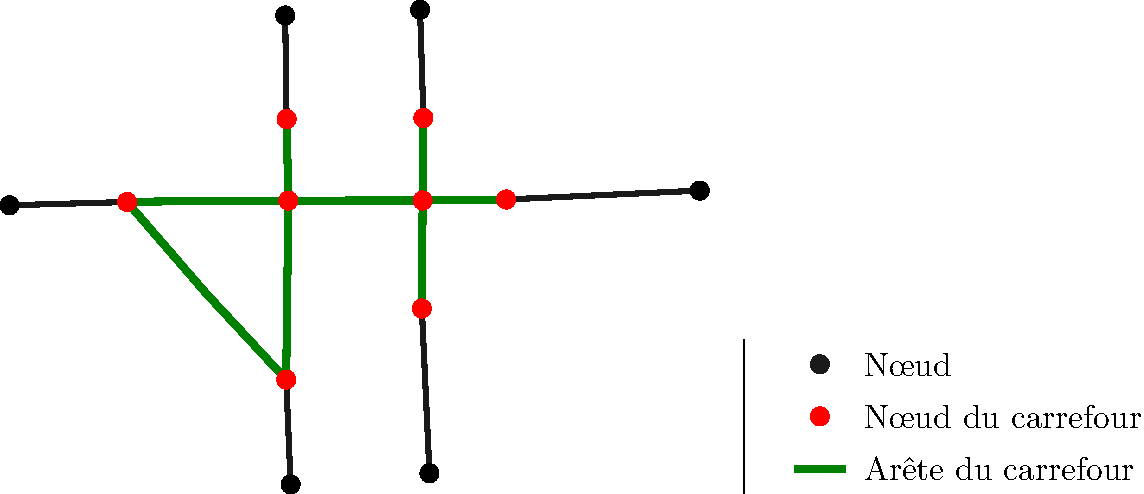
\includegraphics[width=\textwidth]{images/modelisation/segmentation/segmentation-step4.pdf}
        \caption{Résultat de la seconde étape d'assemblage des carrefours de gauche.\label{fig:modelisation_segmentation_step4}}
    \end{subfigure}
    \caption{Résultat de l'assemblage des carrefours élémentaires. Source: \cite{Favreau2022}.}
    \label{fig:modelisation_segmentation_step3&4}
\end{figure}

\newpar{}

La première étape d'assemblage consiste à identifier des couples de carrefours connectés par un chemin court, et qui ont des arêtes adjacentes orthogonales à ce chemin et portant le même nom de rue (voir figure \ref{fig:modelisation_segmentation_step3}). La seconde étape consiste ensuite à identifier les ensembles de carrefours connectés par un cycle court, et de les aggréger en carrefours fonctionnels. Cela nous permet de prendre en compte les carrefours complexes avec des voies de tourne-à-droite, ou des carrefours comportant plusieurs routes internes (voir figure \ref{fig:modelisation_segmentation_step4}). 

\newpar{}

Dans ces deux étapes d'assemblage, la notion de "court" est construite proportionnelement à la largeur de la voie, et en considérant la sémantique des arêtes appartenant au carrefour. Par exemple, si une arête est labellisée comme partie d'un carrefour, alors sa longueur est diminuee. Le chemin résultant est comparé à la largeur de la voie (voir \ref{sec:implementation_segmentation}).

\subsubsection{Segmentation des branches}

\begin{figure}
    \centering
    \resizebox{15cm}{!}{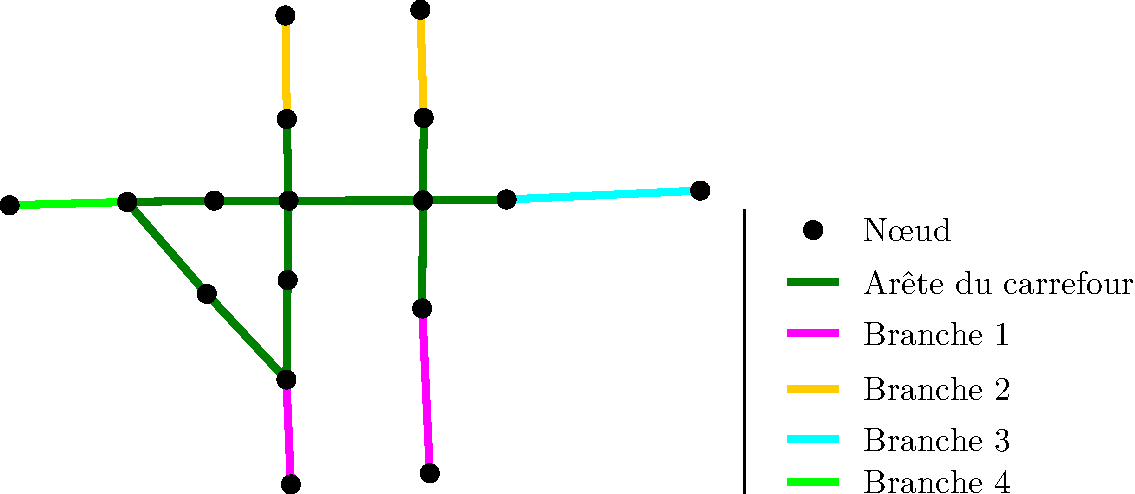
\includegraphics{images/modelisation/segmentation/segmentation-step5.pdf}}
    \caption{Segmentation des branches depuis le carrefour fonctionnel de la figure \ref{fig:modelisation_segmentation_step4} et utilisant les noms de rue donnés en figure {\ref{fig:modelisation_segmentation_step1}}. Source: \cite{Favreau2022}.}
    \label{fig:modelisation_segmentation_step5}
\end{figure}

Enfin, si la chaussée est complexe, il peut arriver que les branches d'un carrefour soit composées de plusieurs arêtes, par exemple en présence d'un séparateur de voies ou d'un îlot. La dernière étape de la segmentation consiste à regrouper les arêtes par branches en utilisant leurs informations géométriques et sémantiques (voir figure \ref{fig:modelisation_segmentation_step5}).

\subsection{Détails du processus de segmentation}

Le processus décrit dans la suite repose sur trois paramètres permettant à l'utilisateur de piloter la segmentation:

\begin{itemize}
    \item $\mathcal{C}_0$ pour ajuster l'échelle du carrefour élémentaire. Appliqué comme coefficient à la largeur de la voie pour moduler la distance maximale pour laquelle un nœud est considéré comme un nœud de bordure d'un carrefour donnée.
    \item $\mathcal{C}_1$ pour ajuster l'échelle de la première fusion des carrefours. Appliqué comme coefficient à la largeur de la voie pour pour moduler la distance maximale de fusion de deux carrefours élémentaires.
    \item $\mathcal{C}_2$ pour ajuster l'échelle de l'assemblage final des carrefours complexes. Appliqué comme coefficient à la largeur de la voie pour pour moduler la longueur maximale du lien qui connecte deux carrefours fonctionnels.
\end{itemize}

\subsubsection{Probabilité d'appartenance à un carrefour ou sa bordure}

Pour modéliser la probabilité qu'un nœud ou une arête appartienne à un carrefour et la probabilité qu'un nœud appartienne à une bordure de carrefour, nous propose d'utiliser une représentation floue: \textit{oui fort}, \textit{oui modéré}, \textit{oui faible}, \textit{incertain}, \textit{non faible}, \textit{non modéré}, \textit{non fort}. Une série de règles est alors utilisée pour transformer la sémantique d'\gls{osm} en incertitude:

\begin{itemize}
    \item  les arêtes labellisées comme carrefour appartiennent à un carrefour (\textit{oui fort}),
    \item  les nœuds labellisés comme passages piétons appartiennent à la bordure d'un carrefour  (\textit{oui fort}),
    \item  les nœuds qui correspondent à un feu de signalisation, un panneau stop ou un cédez-le-passage sont appartiennent probablement à la bordure d'un carrefour (\textit{oui modéré}),
    \item  les nœuds avec une cardinalité supérieure ou égale à quatre sont des nœuds internes à un carrefour (\textit{oui fort}),
    \item  les nœuds avec une cardinalité égale à trois et dont les noms des voies adjacentes ne sont pas uniques appartiennent probablement à un carrefour (\textit{oui modéré}).
\end{itemize}

\newpar{}

Ces règles permettent d'associer une probabilité d'appartenance à certains nœuds, et donc d'initier et guider la segmentation des intersections en considérant une projection synthétique de la sémantique initiale dans un espace simplifié.

\subsubsection{Segmentation en carrefours élémentaires}

Chaque nœud appartenant à un carrefour (\textit{faible oui} ou supérieur), ou faisant partie d'une arête appartenant à un carrefour (\textit{faible oui} ou supérieur) est considéré comme un \emph{nœud graine}. À partir de chacun de ces nœuds, on propage la construction d'une région le long des chemins adjacents, en intégrant un chemin uniquement s'il atteint un nœud identifié comme possible bordure du carrefour, et à une distance raisonnable, en fonction de la largeur des voies autour du nœud initial.

\newpar{}

Si un possible nœud de bordure identifié n'est pas fortement considéré comme faisant partie de la bordure (par exemple si c'est un feu de signalisation), la recherche est poursuivie le long du chemin, au cas où un nœud de bordure fortement considéré soit présent un peu plus loin.

\begin{figure}
    \centering
    \resizebox{15cm}{!}{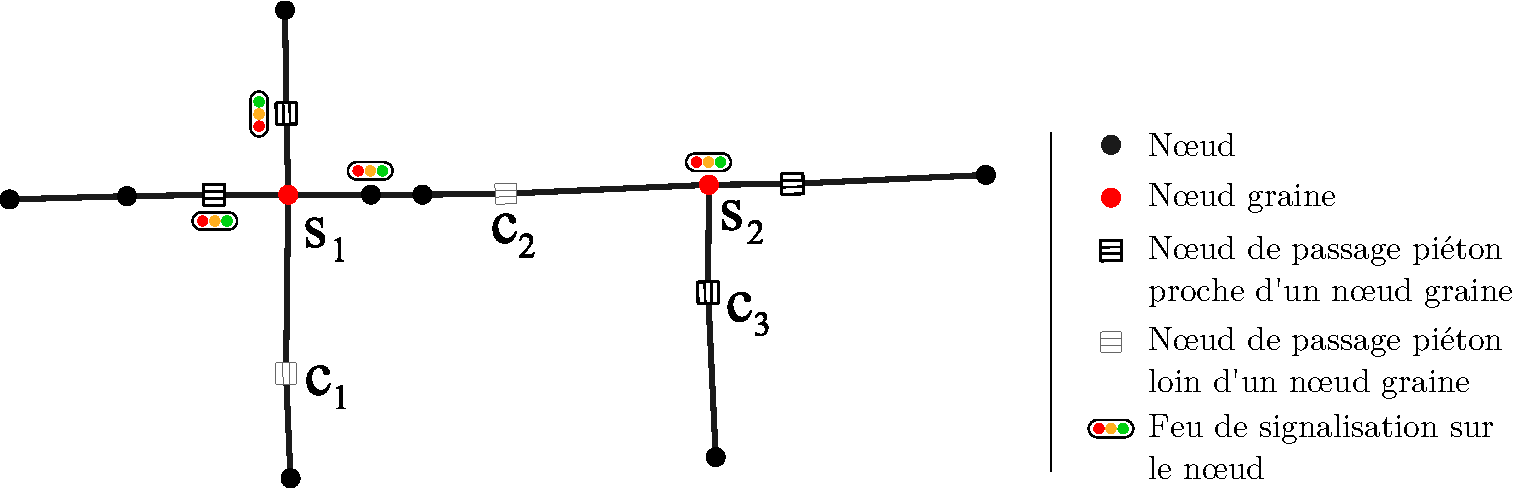
\includegraphics{images/modelisation/segmentation/segmentation-details.pdf}}
    \caption{Deux nœuds graines où des régions élémentaires seront calculées. Source: \cite{Favreau2022}.}
    \label{fig:modelisation_boundarySelection}
\end{figure}

\newpar{}

La figure~\ref{fig:modelisation_boundarySelection} illustre ce processus avec deux nœuds nœuds graines, avec un ensemble de configurations représentatives: 

\begin{itemize}
    \item Le niveau de détails peut varier dans la modélisation: un carrefour ($s_2$) a une description synthétique de l'infrastructure de signalisation, tandis que l'autre carrefour ($s_1$) en propose une description plus précise, chaque feu de signalisation étant localisé sur une route.
    \item Certains passages piétons ($c_1$ et $c_2$) sont éloignés des carrefours et pourraient ne pas être considérés comme des nœuds de bordure.
\end{itemize}

\newpar{}

La proposition que nous avons faite pour la sélection des graines permet aux deux niveaux de détail (détaillé avec $s_1$ et peu détaillé avec $s_2$) d'être pris en compte, étant donné que seule la topologie du graphe et le nom des voies est considérée.

\newpar{}

La transformation de la sémantique d'\gls{osm} en degrés d'appartenance à la bordure nous permet de finement contrôler l'algorithme pour générer des carrefours élémentaires sans se préoccuper de la sémantique des nœuds. Ainsi, le carrefour construit depuis la graine $s_1$ (figure \ref{fig:modelisation_boundarySelection}) sera composé de trois chemins: deux pour les passages piétons associés aux feux de signalisation, et un pour le feu de signalisation sans passage piétons.

\newpar{}

Un possible nœud de bordure $b$ est considéré comme un nœud de bordure d'un carrefour initié par un nœud graine $s$ si il satisfait les condition données par la formule~\ref{eq:0001}, où  $\mathrm{length}(\cdot, \cdot)$ est la longueur du chemin entre $b$ et $s$, $\mathcal{C}_0$ est un paramètre de notre méthode, $E_s$ est un ensemble d'arêtes qui contient $s$, et $w_e$ est une estimation de la largeur des voies.

\begin{equation}
 \mathrm{length}(b, s) \leq \mathcal{C}_0 \max_{e \in E_s} w_e
 \label{eq:0001}
\end{equation}

En pratique, nous estimons la largeur des voies en utilisant une largeur typique pour chaque type de route (3 mètres pour une voie dans un tronçon contenant \osmkey{highway}=\osmvalue{primary}, 2.75 m pour une voie dans un tronçon contenant \osmkey{highway}=\osmvalue{secondary}, etc.). Nous avons également noté que $\mathcal{C}_0=2$ donne de bons résultats dans les centres historiques européens.

\newpar{}

Dans la sélection proposée dans la figure \ref{fig:modelisation_boundarySelection}, $c_1$ et $c_2$ sont considérés comme ne faisant pas partie des carrefours, mais $c_3$ fait partie du carrefour partant de $s_2$.

Si la rue qui connecte $s_1$ à $s_2$ avait été moins large, l'algorithme n'aurait pas considéré $c_3$ comme un des passages piétons proches. De la même manière, si cette rue avait été plus large, $c_1$ aurait rejoint la liste des passages piétons proches du carrefour.

\subsubsection{Fusionner les carrefours élémentaires en utilisant la géométrie et la sémantique}

Les carrefours élémentaires dans le même voisinage sont alors fusionnés en considérant la géométrie de leurs arêtes adjacentes.

Nous comparons pour chaque paire de carrefours élémentaires $i_1$ et $i_2$ la distance euclidienne 
$|s(i_1), s(i_2)$ entre les graines $s(\cdot)$ avec une mesure de proximité donné dans la formule (\ref{eq:0002}), où $\mathcal{C}_1$ est un paramètre de notre méthode, $w(i)$ est la largeur maximum des rues dans $i$, et $\alpha_{i_1, i_2} \in \{ 1, \frac{1}{2} \}$ en fonction de la présence d'un possible nœud de bordure dans le chemin qui connecte $i_1$ et $i_2$.

\begin{equation}
 p_{i_1, i_2} = \mathcal{C}_1 \alpha_{i_1, i_2} \mathrm{max} \{ w(i_1), w(i_2) \}
 \label{eq:0002}
\end{equation}

La paire de carrefours est alors considérée en fonction de cette proximité:
\begin{itemize}
    \item si $|s(i_1), s(i_2) > p_{i_1, i_2}$, les deux carrefours ne sont pas voisins,
    \item si $|s(i_1), s(i_2) \leq \frac{1}{2} p_{i_1, i_2}$, les deux carrefours élémentaires sont considérés comme faisant partie du même carrefour fonctionnel,
    \item entre ces deux valeurs, on considère les angles et noms des arêtes adjacentes pour décider si les deux carrefours élémentaires font partie du même carrefour fonctionnel. Pour chaque paire de carrefours voisins, on identifie les paires d'arêtes adjacentes portant le même nom, qui sont orientées dans une direction similaire (avec un angle relatif inférieur à 90°), et dont l'orientation relative au segment défini par les graines des deux carrefours est significativement différent (d'un angle supérieur à 45°). Si une telle paire d'arêtes existe, alors les deux carrefours élémentaires font parties du même carrefour fonctionnel. La figure \ref{fig:modelisation_elementary_edges_relative_angle} illustre ce calcul en montrant les deux carrefours élémentaires avec deux paires d'arêtes adjacentes, chacune dans la configuration attendue pour fusionner les carrefours.
\end{itemize}

\newpar{}

En pratique, nous avons noté que $\mathcal{C}_1=2$  donne de bons résultats dans les centre historiques européens.

\newpar{}

Une nouvelle région est ainsi créé en assemblant tous les nœuds et arêtes qui constituent les carrefours initiaux, et en ajoutant les nœuds et arêtes qui constituent le chemin qui connecte les carrefours fusionnés.

\begin{figure}
    \centering
    \resizebox{15cm}{!}{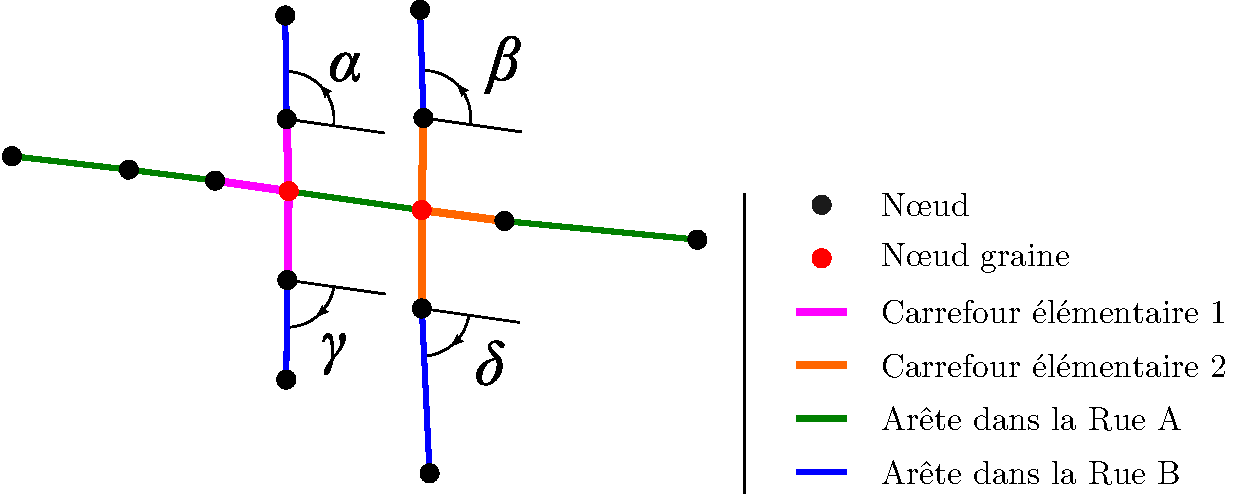
\includegraphics{images/modelisation/segmentation/angles-merge.pdf}}
    \caption{
        Deux carrefours élémentaires dont la proximité entre les nœuds graines nécessite la prise en compte de la configuration des arêtes adjacentes. Ces deux carrefours élémentaires ont deux paires d'arêtes adjacentes ($\{\alpha, \beta\}$ et $\{\gamma, \delta\}$) avec le même nom, des directions consistantes, et des directions significativement différentes au regard du segment défini par les deux graines initiales. Source: \cite{Favreau2022}.}
    \label{fig:modelisation_elementary_edges_relative_angle}
\end{figure}

\subsubsection{Assembler les carrefours}

Une fois que tous les carrefours ont été identifiés et fusionnés par sémantique, ils sont assemblés en carrefours fonctionnels.

\newpar{}

La première étape consiste à identifier toutes les composantes connexes du complémentaire des carrefours précédemment calculés. Ces composantes associées constituent les régions des possibles liens entre les différents carrefours. Dans chacune de ces composantes associées, nous identifions l'ensemble des chemins de liaisons, par exemple les chemins qui connectent deux carrefours distincts.

\newpar{}

Pour piloter la taille des carrefours générés, on définit pour un chemin de liaison $k$ une longueur adaptée définie par la formule \ref{eq:0003}, en fonction de la probabilité qu'il appartienne à un carrefour. Pour cela, on pondère la longueur $\mathrm{length}(k)$ du lien, où $E_k$ est l'ensemble des arêtes de $k$, $n_k$ est le nombre de nœuds dans $k$ dont la cardinalité est supérieure à trois, et $p_e=\frac{1}{2}$ si $e$ est labellisé comme faisant partie d'un carrefour, et $1$ sinon.

\begin{equation}
 \mathrm{length}'(k) = \frac{\sum_{e \in E_k}\mathrm{length}(e) p_e}{\log e^{n_k +1}}
 \label{eq:0003}
\end{equation}

Ensuite, on cherche l'ensemble des cycles qui contiennent une alternance de carrefours et de chemins de liaison, en conservant dans le processus une boucle $l$ si elle satisfait les deux conditions suivantes, pilotées par un paramètre $\mathcal{C}_2$.
D'abord, on sélectionne uniquement les chemins de liaison courts qui vérifie la formule ref{eq:0004}, où $w_k$ est la largeur maximum des voies dans $k$.

\begin{equation}
\mathrm{length}'(k) \leq w_k \mathcal{C}_2
\label{eq:0004}
\end{equation}

À partir de ces chemins de liaison, on sélectionne uniquement les cycles courts, en utilisant $\mathcal{C}_2$ comme paramètre de notre méthode, comme décrit par la formule \ref{eq:0005}, où $L_l$ est l'ensemble des chemins de liaison au sein de $l$.

\begin{equation}
\sum_{k \in L_l} \mathrm{length}'(k) \leq \mathrm{max}_{i \in I_l}\{w_i\} \pi \mathcal{C}_2
\label{eq:0005}
\end{equation}

En pratique, nous avons noté que $\mathcal{C}_2=4$ donne de bons résultats dans les centres historiques européens, quand le paramètre pourrait être augmenté pour capturer des carrefours plus importants, en particulier autour des voies express et des autoroutes.

\newpar{}

Les carrefours fonctionnels sont alors le résultat de l'assemblage des carrefours et des chemins de liaison de ces cycles.

\newpar{}

L'approche que nous proposons a l'avantage de gérer à la fois les carrefours complexes contenant des voies de tourne-à-droite (voir figure~\ref{fig:modelisation_segmentation_step4}), les carrefours complexes qui contiennent des polylignes décrivant les chemins internes du carrefour, mais aussi les ronds-points ( voir figure~\ref{fig:modelisation_roundAbout}).

\begin{figure}
    \centering
    \begin{subfigure}[t]{\columnwidth}
        \resizebox{15cm}{!}{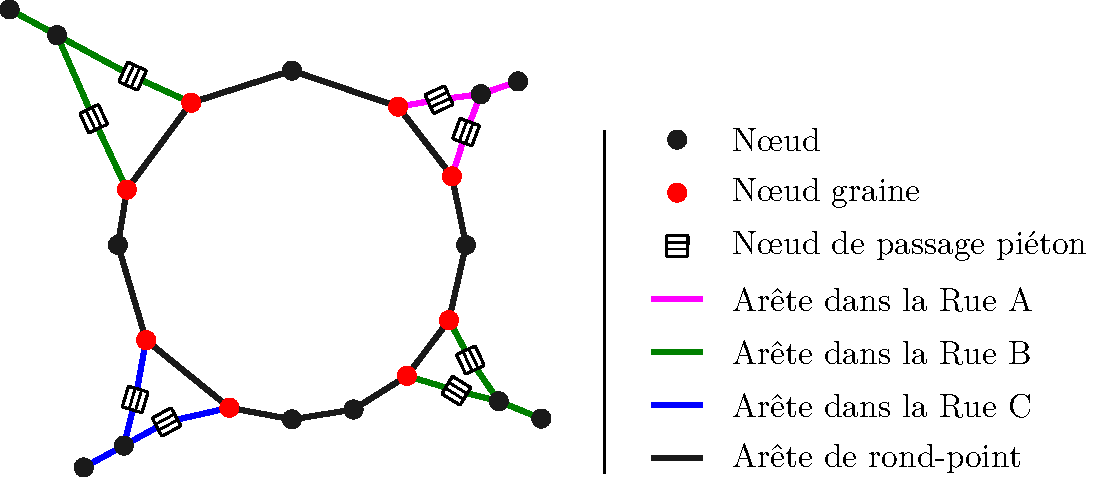
\includegraphics{images/modelisation/segmentation/rond-point.pdf}}
        \caption{Graphe initial où trois rues sont reliées par un rond-point.}
    \end{subfigure}
    \begin{subfigure}[t]{\columnwidth}
        \resizebox{15cm}{!}{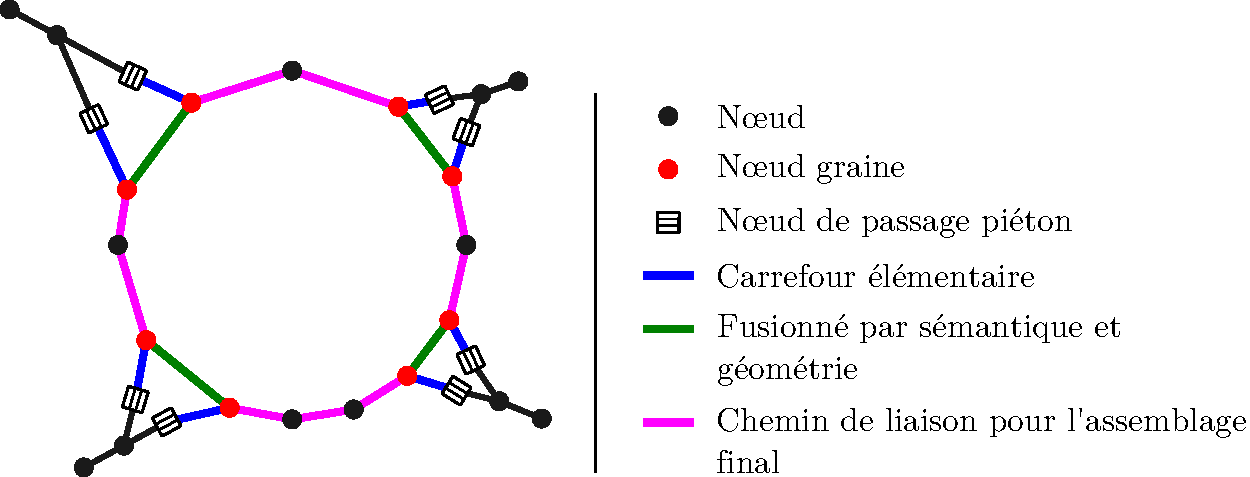
\includegraphics{images/modelisation/segmentation/rond-point-1.pdf}}
        \caption{Transformation pas-à-pas du rond-point en carrefour. Après avoir identifié les huit nœuds graines, chaque carrefour élémentaire est construit, ajoutant un chemin vers le passage piéton le plus proche. Chaque paire de carrefours ayant une voie adjacente portant le même nom de rue, elles sont assemblées en quatre carrefours. Enfin, une boucle est identifiée en connectant ces carrefours le long du chemin du rond-point.}
    \end{subfigure}
    \caption{Illustration du processus dans un rond-point. Source: \cite{Favreau2022}.}
    \label{fig:modelisation_roundAbout}
\end{figure}

\subsubsection{Identification des branches}

\newpar{}

Enfin, pour chaque carrefour assemblé de cette manière, on identifie ses banches en construisant une liste de toutes ses arêtes externes connectées à un nœud appartenant à une arête du carrefour. Ces arêtes sont alors assemblées en les groupant ensemble si elles portent le même nom et sont orientés dans une direction similaire (avec un angle relatif inférieur à 90°), comme illustré en figure \ref{fig:modelisation_mergeBranches}.

\begin{figure}
    \centering
    \resizebox{15cm}{!}{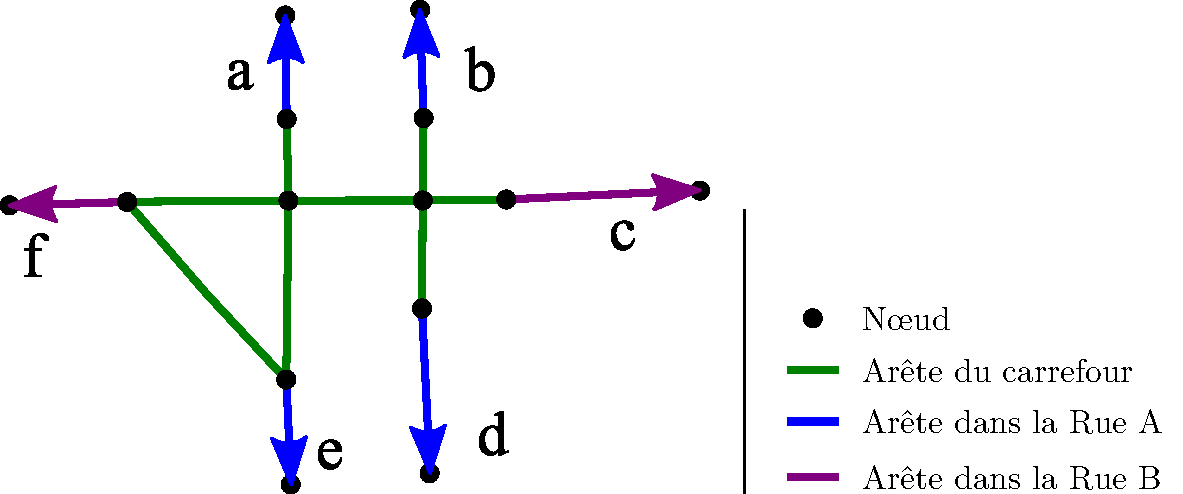
\includegraphics{images/modelisation/segmentation/merge-branches.pdf}}
    \caption{La sémantique de chaque arête adjacente de ce carrefour contient le nom de la rue. On peut alors les grouper en utilisant ces noms et une direction consistante pour calculer les branches correspondantes: $\{a, b\}$, $\{c\}$, $\{d, e\}$, $\{f\}$. Source: \cite{Favreau2022}.}
    \label{fig:modelisation_mergeBranches}
\end{figure}

\subsection{Calcul des informations piétonnes}

À partir d'un carrefour segmenté, il est maintenant possible de déduire des informations piétonnes utiles pour l'instanciation de CrModel, notamment les trottoirs, les îlots, et les traversées de branches. Ces étapes sont détaillées dans les sous-parties suivantes.

\subsubsection{Aggrégation des trottoirs}

\begin{figure}
    \centering
    \resizebox{15cm}{!}{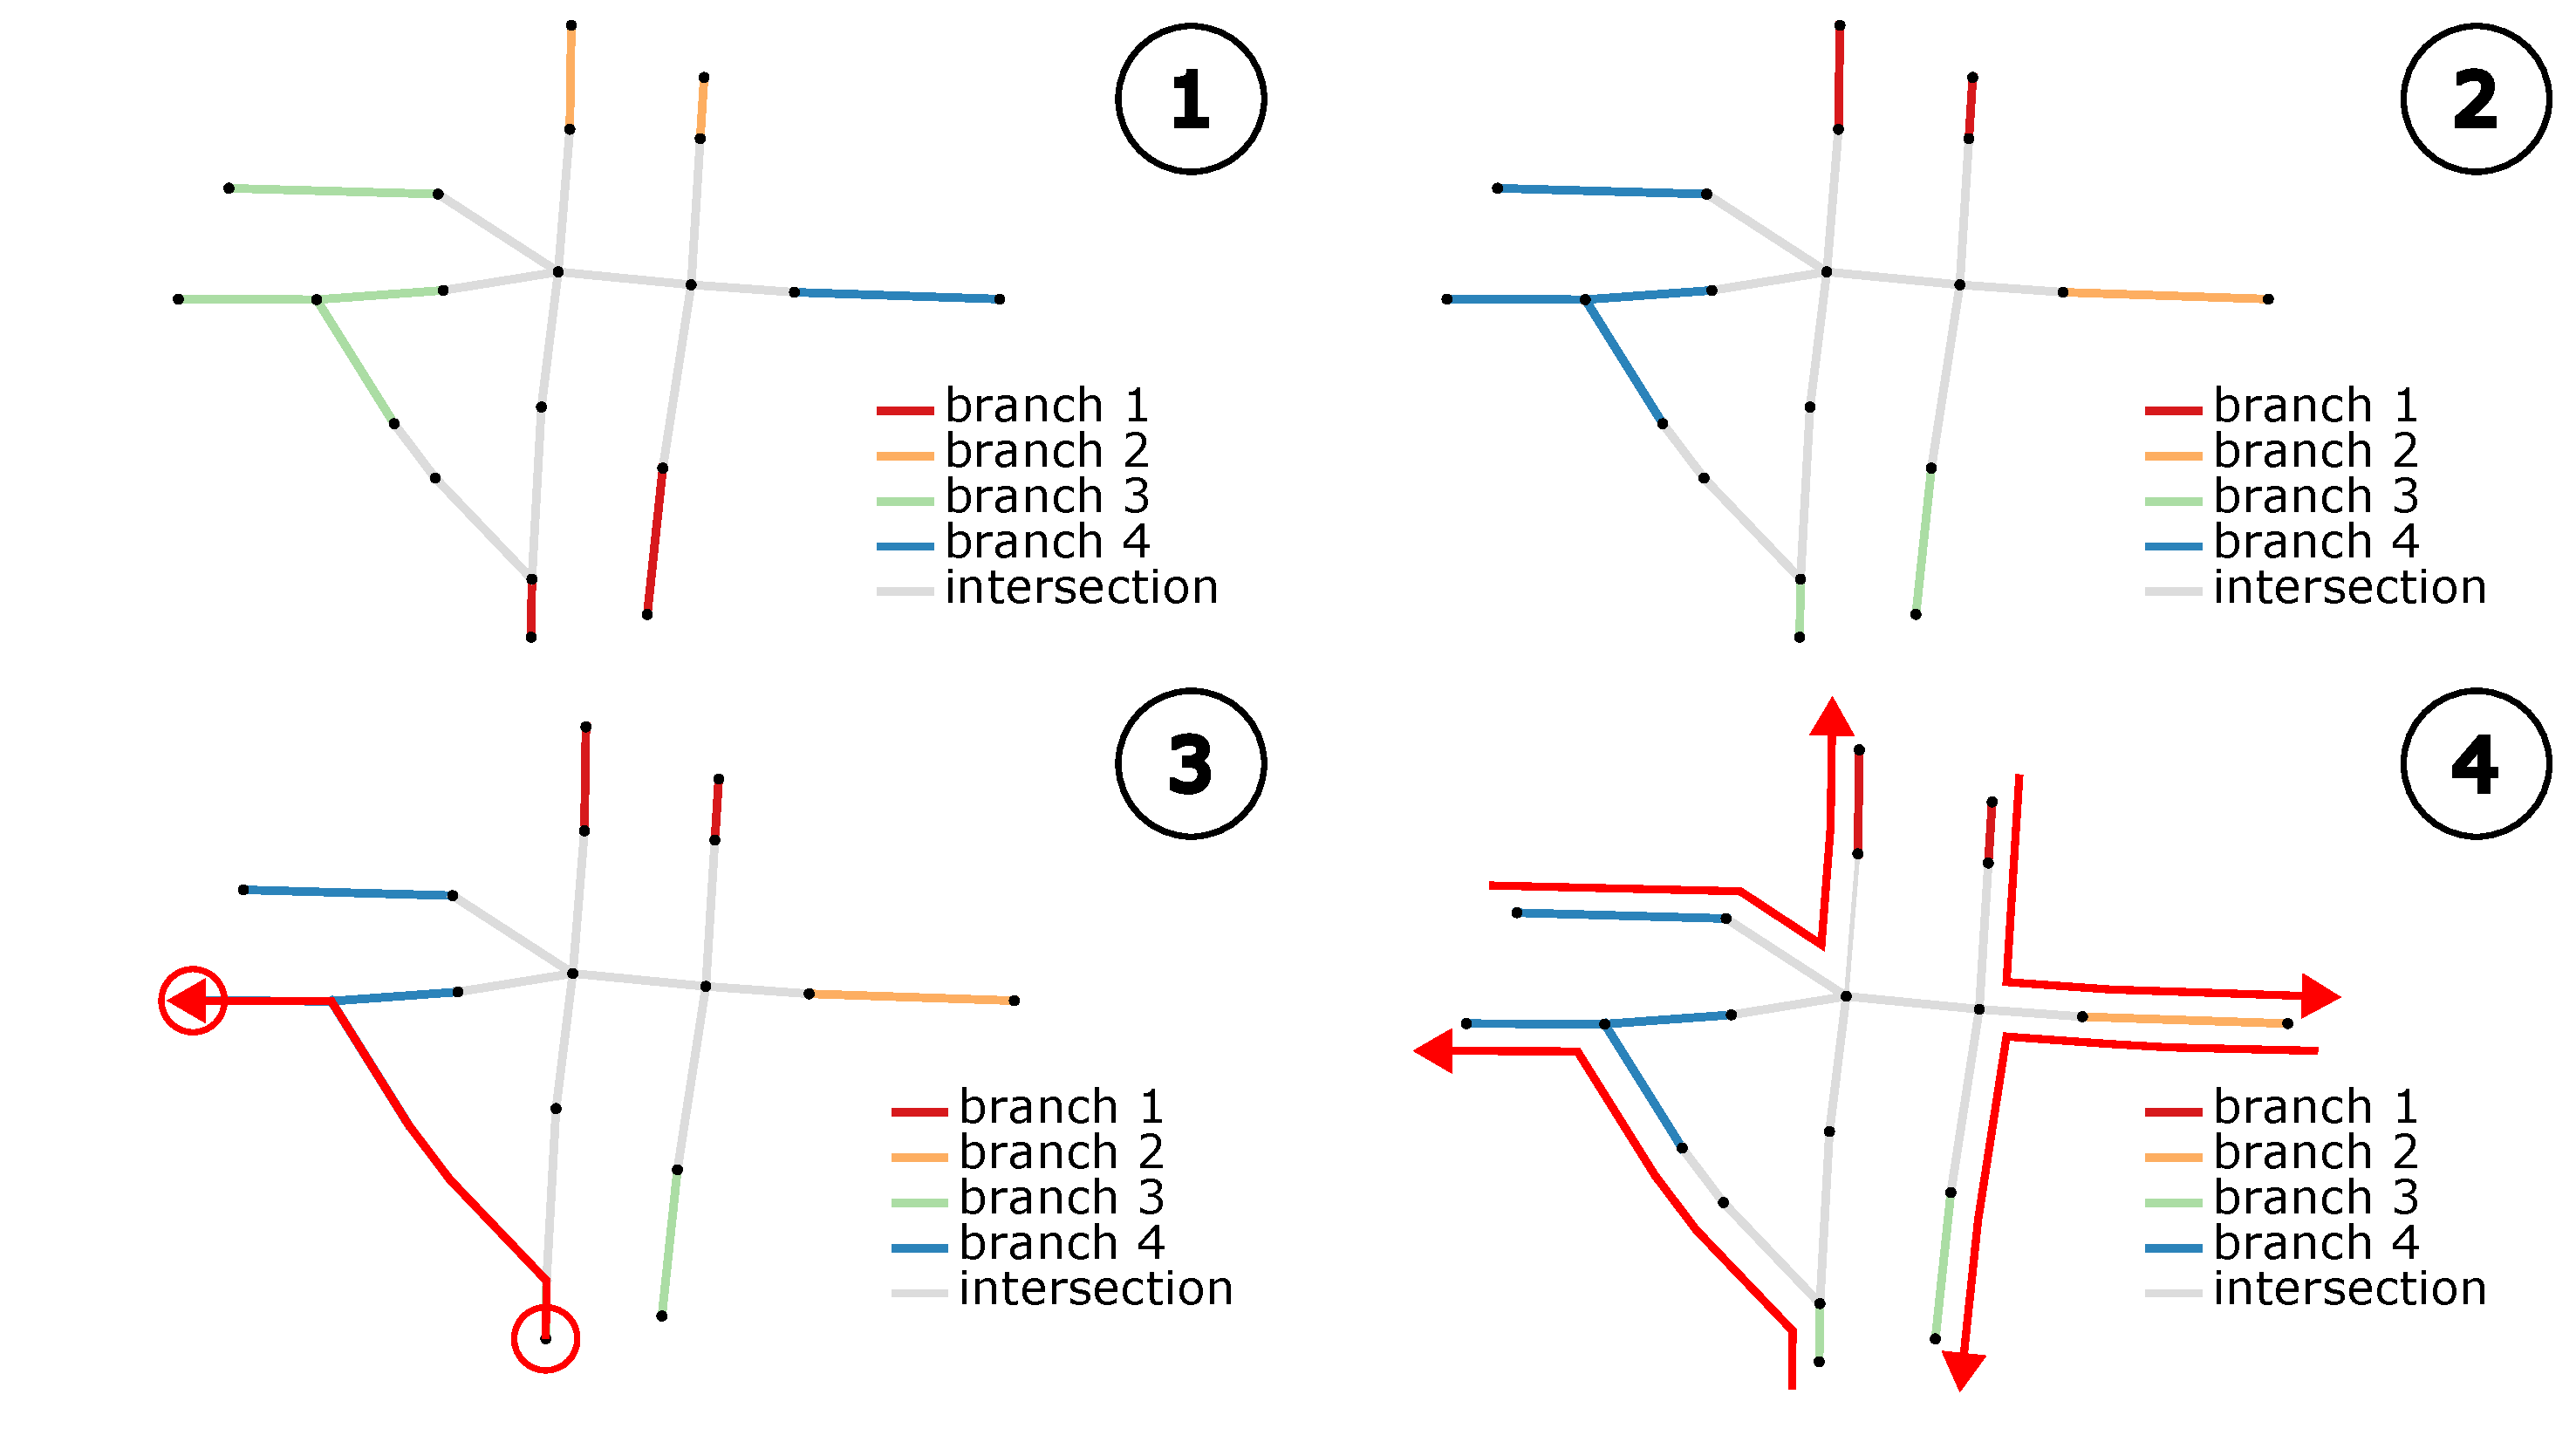
\includegraphics{images/modelisation/calcul_pieton/sidewalks.pdf}}
    \caption{Étapes de génération des trottoirs. Source: \cite{Kalsron2022}.}
    \label{fig:modelisation_calcul_pieton_trottoirs}
\end{figure}

Dans \gls{osm}, les trottoirs identifiés sous forme de sémantique sur le réseau routier ne sont pas aggrégés en une entité unique: chaque tronçon de route indique s'il présente ou non un trottoir à sa droite ou à sa gauche. Si l'on veut considérer une entité trottoir complète, il est nécessaire d'aggréger les tronçons correspondants et déterminer de quel côté le trottoir est situé.

La génération est réalisée de la manière suivante: d'abord, les branches issues de la segmentation (voir figure \ref{fig:modelisation_segmentation_step5}) ne sont pas ordonnées, donc nous les ordonnons dans le sens des aiguilles d'une montre (voir figure \ref{fig:modelisation_calcul_pieton_trottoirs}.2). Pour chaque branche du carrefour, une par une dans le sens des aiguilles d'une montre, on part du nœud situé à l'extrémité de l'arête la plus à droite et on parcours le graphe en tournant toujours à gauche jusqu'à atteindre une seconde extrêmité (voir figure \ref{fig:modelisation_calcul_pieton_trottoirs}.3). Le chemin traversé correspond alors à un trottoir (voir figure \ref{fig:modelisation_calcul_pieton_trottoirs}.4). Si l'arête est traversée dans sa direction, le trottoir est situé à sa gauche, sinon il est situé à sa droite. Si aucune sémantique n'indique l'absence de trottoir, on considère qu'il est présent. Nous avons fait ce choix car la majorité des villes ont des trottoirs, et la donnée \gls{osm} n'est pas encore suffisamment renseignée sur la sémantique associée.

\subsubsection{Génération des îlots}

\begin{figure}
    \centering
    \resizebox{15cm}{!}{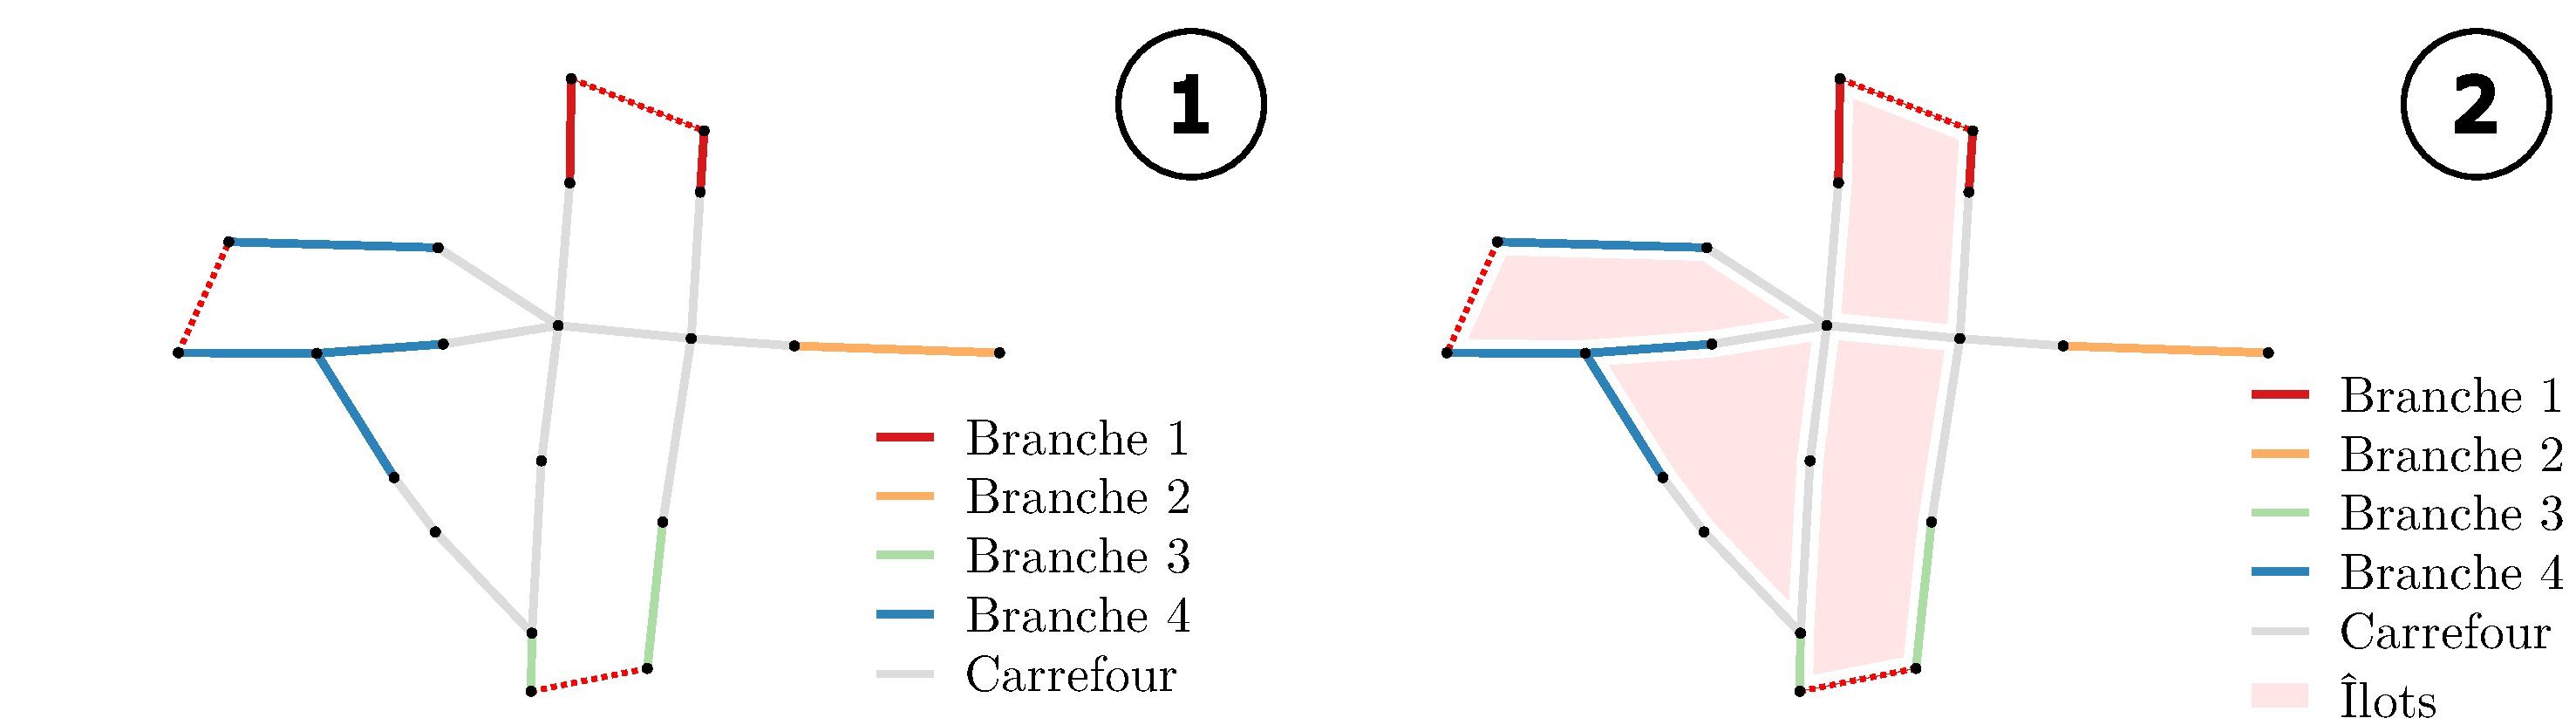
\includegraphics{images/modelisation/calcul_pieton/islands.pdf}}
    \caption{Étapes de génération des îlots. Source: \cite{Kalsron2022}.}
    \label{fig:modelisation_calcul_pieton_ilots}
\end{figure}

En dehors de la clé \osmkey{crossing:island} qui indique la présence d'un îlot au milieu d'une traversée mais dont la présence est marginale, les îlots sont absents de la sémantique d'\gls{osm}. En revanche, l'usage montre que les îlots sont représentés par les faces du graphe routier et peuvent être déduits de cette manière \cite{Vitalis2022}. Pour cela, il faut tout d'abord fermer les branches composées de plusieurs arêtes (voir figure \ref{fig:modelisation_calcul_pieton_ilots}.1) pour obtenir des faces et détecter l'intégralité des îlots (voir figure \ref{fig:modelisation_calcul_pieton_ilots}.2).

\subsubsection{Génération des traversées}

\begin{figure}
    \centering
    \resizebox{15cm}{!}{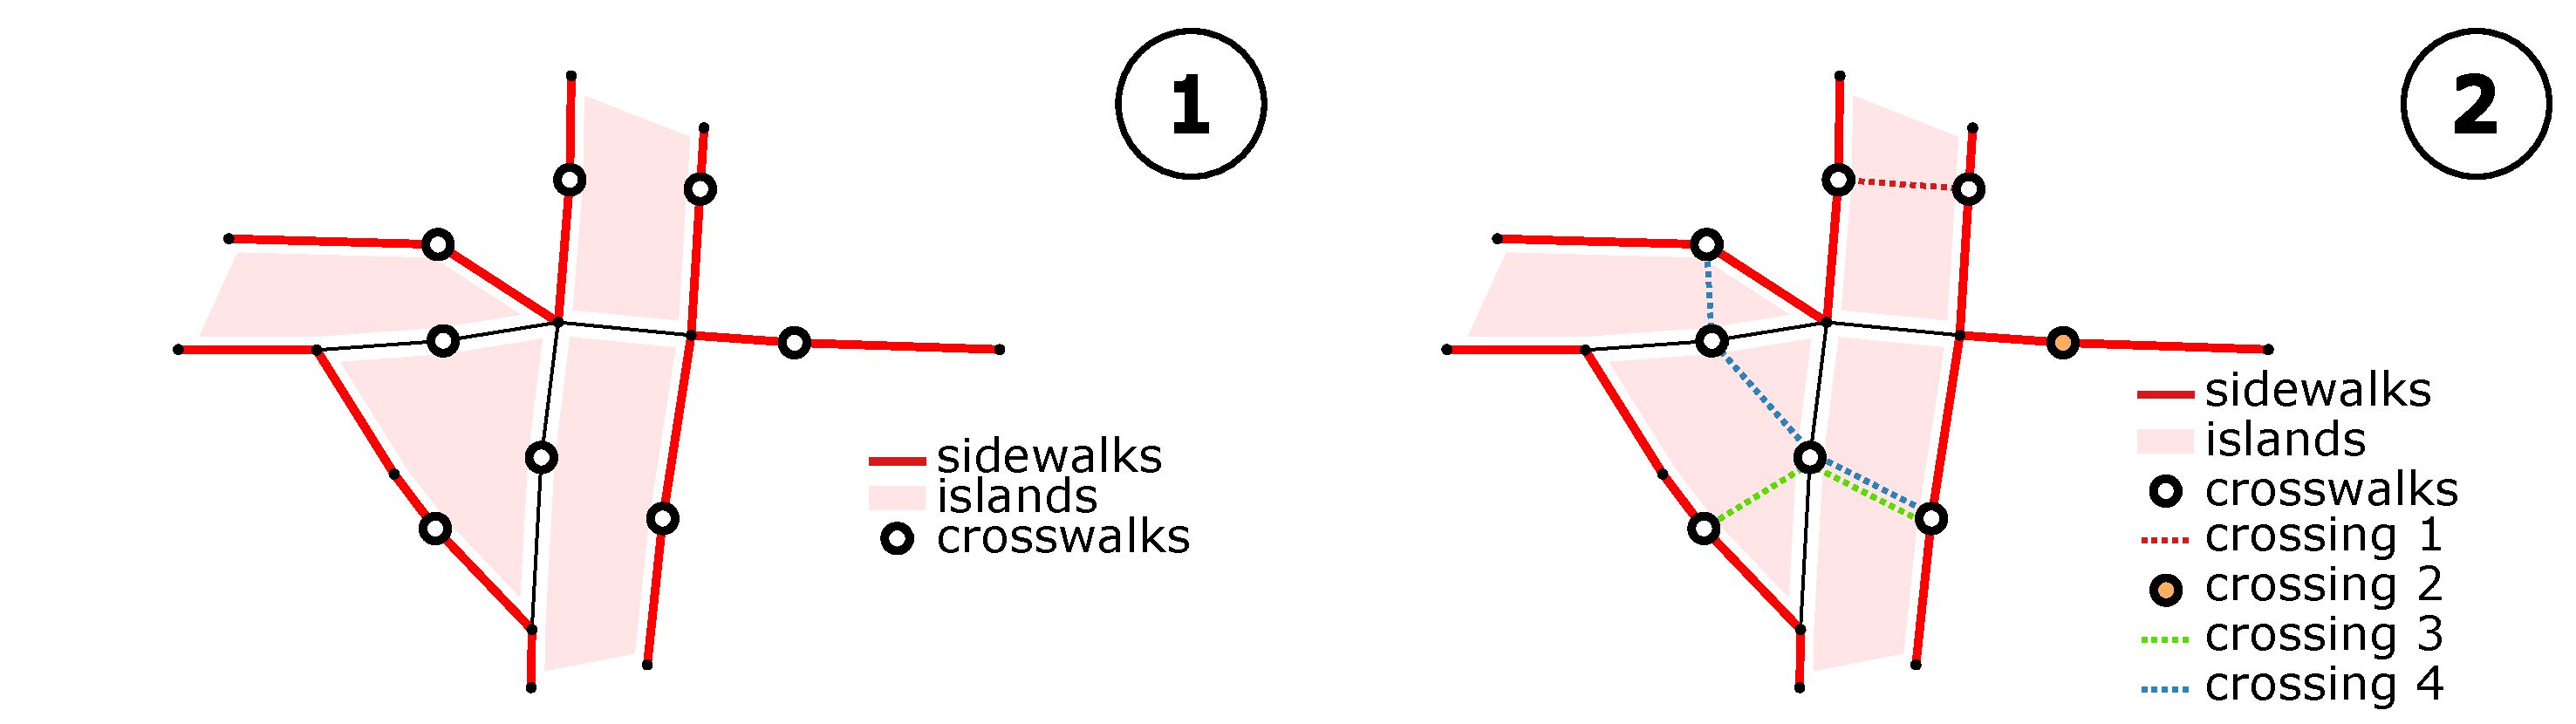
\includegraphics{images/modelisation/calcul_pieton/crossings.pdf}}
    \caption{Étapes de génération des traversées. Source: \cite{Kalsron2022}.}
    \label{fig:modelisation_calcul_pieton_traversees}
\end{figure}

Après avoir généré les trottoirs et les îlots, une traversée correspond à une séquence de passages piétons permettant de traverser d'un trottoir à un autre en passant uniquement par des îlots. On peut alors générer ces traversées en utilisant un graphe dual où les trottoirs et les îlots deviennent des nœuds, et les passages piétons des arêtes. Calculer les traversées revient alors à calculer le chemin le plus court entre deux trottoirs sans passer par un autre trottoir (voir figure \ref{fig:modelisation_calcul_pieton_traversees}).

\section{Conclusion du chapitre}

Dans ce chapitre, nous avons étudié la structure globale du carrefour du point de vue d'un piéton déficient visuel, en nous intéressant dans un premier temps à sa construction topologique, et à son infrastructure d'accessibilité. Les données d'accessibilités existantes étant éparses et hétérogènes, nous avons choisi de travailler sur \gls{osm} en analysant la manière dont les carrefours et l'accessibilité y sont cartographiés.

\newpar{}

Nous avons proposé un modèle de données permettant de représenter la sémantique d'\gls{osm} dans un formalisme objet. Nous l'avons appliqué à un modèle de données permettant de représenter un carrefour du point de vue du piéton, en modélisant notamment les traversées. Nous détaillons par la suite les processus permettant d'instancier ce modèle depuis \gls{osm} en segmentant son graphe routier pour y détecter les carrefours et leurs attributs. L'implémentation et l'évaluation des processus présentés sont détaillées respectivement en chapitres \ref{chap:implementation} et \ref{chap:evaluation}.

\newpar{}

Le modèle présenté peut avoir de nombreux usages, de la généralisation du carrefour à sa représentation sous une autre forme. Le chapitre suivant se concentre sur ce deuxième cas, en s'intéressant à la description textuelle des carrefours.